\documentclass[11pt]{article}

% Shared notes settings for Applied Machine Learning lectures (UPES).
% Keep this file free of \documentclass to allow reuse via \input.

\usepackage[utf8]{inputenc}
\usepackage[T1]{fontenc}
\usepackage{lmodern}          % scalable T1 fonts; without this pdflatex falls back
\input{glyphtounicode}        % to bitmapped EC Type 3 and the PDFs are neither
\pdfgentounicode=1            % searchable nor screen-reader friendly
\usepackage[a4paper,margin=1in]{geometry}
\usepackage{hyperref}
\usepackage{xurl}
\usepackage{booktabs}
\usepackage{amsmath}
\usepackage{amssymb}
\usepackage{listings}
\usepackage{xcolor}
\usepackage{enumitem}
\usepackage{parskip}

% Code listings (Python-oriented for this subject).
\lstset{
  language=Python,
  basicstyle=\ttfamily\small,
  keywordstyle=\color{blue},
  commentstyle=\color{gray},
  stringstyle=\color{teal},
  showstringspaces=false,
  columns=fullflexible,
  frame=single,
  framerule=0.2pt,
  breaklines=true
}

\setlist[itemize]{topsep=0.3em,itemsep=0.2em}
\setlist[enumerate]{topsep=0.3em,itemsep=0.2em}

% Simple per-section source line.
\newcommand{\notesources}[1]{\par\noindent{\small\color{gray}\textit{Sources:} \sloppy #1\par}}

% Unit-wise source strings for this subject (used by slides + notes).
% Path is relative to the lecture `latex/` folder (the compilation CWD).
\IfFileExists{../../../_shared/aml-sources.tex}{%
  % Source strings for Applied Machine Learning (CSAI2017P) — used by slides + notes.
% Prescribed texts and reference books are taken from the course syllabus.
% Support texts are the author-hosted open-access editions:
%   statlearning.com            (ISL with Python)
%   probml.github.io/pml-book   (Murphy, Probabilistic Machine Learning)
%   d2l.ai                      (Dive into Deep Learning)
%   mml-book.github.io          (Mathematics for Machine Learning)

\newcommand{\AMLRepoURL}{https://github.com/tali7c/Applied-Machine-Learning}

% --- prescribed -------------------------------------------------------------
\newcommand{\AMLPrescribed}{%
M\"uller and Guido, \textit{Introduction to Machine Learning with Python}, O'Reilly, 2016.;%
Bishop, \textit{Pattern Recognition and Machine Learning}, Springer, 2006.;%
Murphy, \textit{Machine Learning: A Probabilistic Perspective}, MIT Press, 2012.;%
Han, Kamber and Pei, \textit{Data Mining: Concepts and Techniques} (3e), Morgan Kaufmann, 2012.%
}

% --- unit-wise ---------------------------------------------------------------
\newcommand{\AMLUnitISources}{%
M\"uller and Guido, \textit{Introduction to Machine Learning with Python}, Ch. 1.;%
Bishop, \textit{Pattern Recognition and Machine Learning}, Ch. 1.;%
Murphy, \textit{Probabilistic Machine Learning: An Introduction}, MIT Press, 2022, Ch. 1.;%
Mitchell, \textit{Machine Learning}, McGraw Hill, 1997, Ch. 1.;%
Scikit-learn documentation, accessed 2026-08-04.%
}

\newcommand{\AMLUnitIISources}{%
Bishop, \textit{Pattern Recognition and Machine Learning}, \S1.5, \S4.3, \S7.1.;%
Zhang, Lipton, Li and Smola, \textit{Dive into Deep Learning}, \S3.4.;%
Shalev-Shwartz and Ben-David, \textit{Understanding Machine Learning}, Ch. 15.;%
Murphy, \textit{Probabilistic Machine Learning: An Introduction}, Ch. 5.%
}

\newcommand{\AMLUnitIIISources}{%
Zhang, Lipton, Li and Smola, \textit{Dive into Deep Learning}, Ch. 12 (Optimization Algorithms).;%
Deisenroth, Faisal and Ong, \textit{Mathematics for Machine Learning}, Ch. 7.;%
Kingma and Ba, ``Adam: A Method for Stochastic Optimization,'' ICLR 2015.;%
Ruder, ``An overview of gradient descent optimization algorithms,'' arXiv:1609.04747, 2016.%
}

\newcommand{\AMLUnitIVSources}{%
Han, Kamber and Pei, \textit{Data Mining: Concepts and Techniques} (3e), Ch. 3.;%
M\"uller and Guido, \textit{Introduction to Machine Learning with Python}, Ch. 3--4.;%
James, Witten, Hastie, Tibshirani and Taylor, \textit{An Introduction to Statistical Learning with Python}, Ch. 5--6, 12.;%
Scikit-learn documentation (preprocessing, model selection), accessed 2026-08-04.%
}

\newcommand{\AMLUnitVSources}{%
James et al., \textit{An Introduction to Statistical Learning with Python}, Ch. 3--6.;%
Bishop, \textit{Pattern Recognition and Machine Learning}, Ch. 3.;%
Deisenroth, Faisal and Ong, \textit{Mathematics for Machine Learning}, Ch. 9.;%
M\"uller and Guido, \textit{Introduction to Machine Learning with Python}, \S2.3.%
}

\newcommand{\AMLUnitVISources}{%
Han, Kamber and Pei, \textit{Data Mining: Concepts and Techniques} (3e), Ch. 8--9.;%
James et al., \textit{An Introduction to Statistical Learning with Python}, Ch. 8--9.;%
Bishop, \textit{Pattern Recognition and Machine Learning}, Ch. 4--5, 7, 14.;%
Zhang et al., \textit{Dive into Deep Learning}, Ch. 5.%
}

\newcommand{\AMLUnitVIISources}{%
Han, Kamber and Pei, \textit{Data Mining: Concepts and Techniques} (3e), Ch. 10.;%
James et al., \textit{An Introduction to Statistical Learning with Python}, Ch. 12.;%
M\"uller and Guido, \textit{Introduction to Machine Learning with Python}, \S3.5.;%
Ester, Kriegel, Sander and Xu, ``A density-based algorithm for discovering clusters (DBSCAN),'' KDD 1996.%
}

\newcommand{\AMLLabSources}{%
M\"uller and Guido, \textit{Introduction to Machine Learning with Python}, companion notebooks.;%
McKinney, \textit{Python for Data Analysis} (3e), O'Reilly, 2022.;%
Scikit-learn user guide, accessed 2026-08-04.;%
Matplotlib and Seaborn documentation, accessed 2026-08-04.%
}
%
}{%
  % Faculty copies live under `private/` so their compile CWD is different.
  \IfFileExists{../../../../public/_shared/aml-sources.tex}{%
    % Source strings for Applied Machine Learning (CSAI2017P) — used by slides + notes.
% Prescribed texts and reference books are taken from the course syllabus.
% Support texts are the author-hosted open-access editions:
%   statlearning.com            (ISL with Python)
%   probml.github.io/pml-book   (Murphy, Probabilistic Machine Learning)
%   d2l.ai                      (Dive into Deep Learning)
%   mml-book.github.io          (Mathematics for Machine Learning)

\newcommand{\AMLRepoURL}{https://github.com/tali7c/Applied-Machine-Learning}

% --- prescribed -------------------------------------------------------------
\newcommand{\AMLPrescribed}{%
M\"uller and Guido, \textit{Introduction to Machine Learning with Python}, O'Reilly, 2016.;%
Bishop, \textit{Pattern Recognition and Machine Learning}, Springer, 2006.;%
Murphy, \textit{Machine Learning: A Probabilistic Perspective}, MIT Press, 2012.;%
Han, Kamber and Pei, \textit{Data Mining: Concepts and Techniques} (3e), Morgan Kaufmann, 2012.%
}

% --- unit-wise ---------------------------------------------------------------
\newcommand{\AMLUnitISources}{%
M\"uller and Guido, \textit{Introduction to Machine Learning with Python}, Ch. 1.;%
Bishop, \textit{Pattern Recognition and Machine Learning}, Ch. 1.;%
Murphy, \textit{Probabilistic Machine Learning: An Introduction}, MIT Press, 2022, Ch. 1.;%
Mitchell, \textit{Machine Learning}, McGraw Hill, 1997, Ch. 1.;%
Scikit-learn documentation, accessed 2026-08-04.%
}

\newcommand{\AMLUnitIISources}{%
Bishop, \textit{Pattern Recognition and Machine Learning}, \S1.5, \S4.3, \S7.1.;%
Zhang, Lipton, Li and Smola, \textit{Dive into Deep Learning}, \S3.4.;%
Shalev-Shwartz and Ben-David, \textit{Understanding Machine Learning}, Ch. 15.;%
Murphy, \textit{Probabilistic Machine Learning: An Introduction}, Ch. 5.%
}

\newcommand{\AMLUnitIIISources}{%
Zhang, Lipton, Li and Smola, \textit{Dive into Deep Learning}, Ch. 12 (Optimization Algorithms).;%
Deisenroth, Faisal and Ong, \textit{Mathematics for Machine Learning}, Ch. 7.;%
Kingma and Ba, ``Adam: A Method for Stochastic Optimization,'' ICLR 2015.;%
Ruder, ``An overview of gradient descent optimization algorithms,'' arXiv:1609.04747, 2016.%
}

\newcommand{\AMLUnitIVSources}{%
Han, Kamber and Pei, \textit{Data Mining: Concepts and Techniques} (3e), Ch. 3.;%
M\"uller and Guido, \textit{Introduction to Machine Learning with Python}, Ch. 3--4.;%
James, Witten, Hastie, Tibshirani and Taylor, \textit{An Introduction to Statistical Learning with Python}, Ch. 5--6, 12.;%
Scikit-learn documentation (preprocessing, model selection), accessed 2026-08-04.%
}

\newcommand{\AMLUnitVSources}{%
James et al., \textit{An Introduction to Statistical Learning with Python}, Ch. 3--6.;%
Bishop, \textit{Pattern Recognition and Machine Learning}, Ch. 3.;%
Deisenroth, Faisal and Ong, \textit{Mathematics for Machine Learning}, Ch. 9.;%
M\"uller and Guido, \textit{Introduction to Machine Learning with Python}, \S2.3.%
}

\newcommand{\AMLUnitVISources}{%
Han, Kamber and Pei, \textit{Data Mining: Concepts and Techniques} (3e), Ch. 8--9.;%
James et al., \textit{An Introduction to Statistical Learning with Python}, Ch. 8--9.;%
Bishop, \textit{Pattern Recognition and Machine Learning}, Ch. 4--5, 7, 14.;%
Zhang et al., \textit{Dive into Deep Learning}, Ch. 5.%
}

\newcommand{\AMLUnitVIISources}{%
Han, Kamber and Pei, \textit{Data Mining: Concepts and Techniques} (3e), Ch. 10.;%
James et al., \textit{An Introduction to Statistical Learning with Python}, Ch. 12.;%
M\"uller and Guido, \textit{Introduction to Machine Learning with Python}, \S3.5.;%
Ester, Kriegel, Sander and Xu, ``A density-based algorithm for discovering clusters (DBSCAN),'' KDD 1996.%
}

\newcommand{\AMLLabSources}{%
M\"uller and Guido, \textit{Introduction to Machine Learning with Python}, companion notebooks.;%
McKinney, \textit{Python for Data Analysis} (3e), O'Reilly, 2022.;%
Scikit-learn user guide, accessed 2026-08-04.;%
Matplotlib and Seaborn documentation, accessed 2026-08-04.%
}
%
  }{%
    % Question papers live at `private/<family>/<instrument>/`.
    \IfFileExists{../../../public/_shared/aml-sources.tex}{%
      % Source strings for Applied Machine Learning (CSAI2017P) — used by slides + notes.
% Prescribed texts and reference books are taken from the course syllabus.
% Support texts are the author-hosted open-access editions:
%   statlearning.com            (ISL with Python)
%   probml.github.io/pml-book   (Murphy, Probabilistic Machine Learning)
%   d2l.ai                      (Dive into Deep Learning)
%   mml-book.github.io          (Mathematics for Machine Learning)

\newcommand{\AMLRepoURL}{https://github.com/tali7c/Applied-Machine-Learning}

% --- prescribed -------------------------------------------------------------
\newcommand{\AMLPrescribed}{%
M\"uller and Guido, \textit{Introduction to Machine Learning with Python}, O'Reilly, 2016.;%
Bishop, \textit{Pattern Recognition and Machine Learning}, Springer, 2006.;%
Murphy, \textit{Machine Learning: A Probabilistic Perspective}, MIT Press, 2012.;%
Han, Kamber and Pei, \textit{Data Mining: Concepts and Techniques} (3e), Morgan Kaufmann, 2012.%
}

% --- unit-wise ---------------------------------------------------------------
\newcommand{\AMLUnitISources}{%
M\"uller and Guido, \textit{Introduction to Machine Learning with Python}, Ch. 1.;%
Bishop, \textit{Pattern Recognition and Machine Learning}, Ch. 1.;%
Murphy, \textit{Probabilistic Machine Learning: An Introduction}, MIT Press, 2022, Ch. 1.;%
Mitchell, \textit{Machine Learning}, McGraw Hill, 1997, Ch. 1.;%
Scikit-learn documentation, accessed 2026-08-04.%
}

\newcommand{\AMLUnitIISources}{%
Bishop, \textit{Pattern Recognition and Machine Learning}, \S1.5, \S4.3, \S7.1.;%
Zhang, Lipton, Li and Smola, \textit{Dive into Deep Learning}, \S3.4.;%
Shalev-Shwartz and Ben-David, \textit{Understanding Machine Learning}, Ch. 15.;%
Murphy, \textit{Probabilistic Machine Learning: An Introduction}, Ch. 5.%
}

\newcommand{\AMLUnitIIISources}{%
Zhang, Lipton, Li and Smola, \textit{Dive into Deep Learning}, Ch. 12 (Optimization Algorithms).;%
Deisenroth, Faisal and Ong, \textit{Mathematics for Machine Learning}, Ch. 7.;%
Kingma and Ba, ``Adam: A Method for Stochastic Optimization,'' ICLR 2015.;%
Ruder, ``An overview of gradient descent optimization algorithms,'' arXiv:1609.04747, 2016.%
}

\newcommand{\AMLUnitIVSources}{%
Han, Kamber and Pei, \textit{Data Mining: Concepts and Techniques} (3e), Ch. 3.;%
M\"uller and Guido, \textit{Introduction to Machine Learning with Python}, Ch. 3--4.;%
James, Witten, Hastie, Tibshirani and Taylor, \textit{An Introduction to Statistical Learning with Python}, Ch. 5--6, 12.;%
Scikit-learn documentation (preprocessing, model selection), accessed 2026-08-04.%
}

\newcommand{\AMLUnitVSources}{%
James et al., \textit{An Introduction to Statistical Learning with Python}, Ch. 3--6.;%
Bishop, \textit{Pattern Recognition and Machine Learning}, Ch. 3.;%
Deisenroth, Faisal and Ong, \textit{Mathematics for Machine Learning}, Ch. 9.;%
M\"uller and Guido, \textit{Introduction to Machine Learning with Python}, \S2.3.%
}

\newcommand{\AMLUnitVISources}{%
Han, Kamber and Pei, \textit{Data Mining: Concepts and Techniques} (3e), Ch. 8--9.;%
James et al., \textit{An Introduction to Statistical Learning with Python}, Ch. 8--9.;%
Bishop, \textit{Pattern Recognition and Machine Learning}, Ch. 4--5, 7, 14.;%
Zhang et al., \textit{Dive into Deep Learning}, Ch. 5.%
}

\newcommand{\AMLUnitVIISources}{%
Han, Kamber and Pei, \textit{Data Mining: Concepts and Techniques} (3e), Ch. 10.;%
James et al., \textit{An Introduction to Statistical Learning with Python}, Ch. 12.;%
M\"uller and Guido, \textit{Introduction to Machine Learning with Python}, \S3.5.;%
Ester, Kriegel, Sander and Xu, ``A density-based algorithm for discovering clusters (DBSCAN),'' KDD 1996.%
}

\newcommand{\AMLLabSources}{%
M\"uller and Guido, \textit{Introduction to Machine Learning with Python}, companion notebooks.;%
McKinney, \textit{Python for Data Analysis} (3e), O'Reilly, 2022.;%
Scikit-learn user guide, accessed 2026-08-04.;%
Matplotlib and Seaborn documentation, accessed 2026-08-04.%
}
%
    }{%
      % Marking schemes live at `private/solutions/<family>/<id>/latex/`.
      \IfFileExists{../../../../../public/_shared/aml-sources.tex}{%
        % Source strings for Applied Machine Learning (CSAI2017P) — used by slides + notes.
% Prescribed texts and reference books are taken from the course syllabus.
% Support texts are the author-hosted open-access editions:
%   statlearning.com            (ISL with Python)
%   probml.github.io/pml-book   (Murphy, Probabilistic Machine Learning)
%   d2l.ai                      (Dive into Deep Learning)
%   mml-book.github.io          (Mathematics for Machine Learning)

\newcommand{\AMLRepoURL}{https://github.com/tali7c/Applied-Machine-Learning}

% --- prescribed -------------------------------------------------------------
\newcommand{\AMLPrescribed}{%
M\"uller and Guido, \textit{Introduction to Machine Learning with Python}, O'Reilly, 2016.;%
Bishop, \textit{Pattern Recognition and Machine Learning}, Springer, 2006.;%
Murphy, \textit{Machine Learning: A Probabilistic Perspective}, MIT Press, 2012.;%
Han, Kamber and Pei, \textit{Data Mining: Concepts and Techniques} (3e), Morgan Kaufmann, 2012.%
}

% --- unit-wise ---------------------------------------------------------------
\newcommand{\AMLUnitISources}{%
M\"uller and Guido, \textit{Introduction to Machine Learning with Python}, Ch. 1.;%
Bishop, \textit{Pattern Recognition and Machine Learning}, Ch. 1.;%
Murphy, \textit{Probabilistic Machine Learning: An Introduction}, MIT Press, 2022, Ch. 1.;%
Mitchell, \textit{Machine Learning}, McGraw Hill, 1997, Ch. 1.;%
Scikit-learn documentation, accessed 2026-08-04.%
}

\newcommand{\AMLUnitIISources}{%
Bishop, \textit{Pattern Recognition and Machine Learning}, \S1.5, \S4.3, \S7.1.;%
Zhang, Lipton, Li and Smola, \textit{Dive into Deep Learning}, \S3.4.;%
Shalev-Shwartz and Ben-David, \textit{Understanding Machine Learning}, Ch. 15.;%
Murphy, \textit{Probabilistic Machine Learning: An Introduction}, Ch. 5.%
}

\newcommand{\AMLUnitIIISources}{%
Zhang, Lipton, Li and Smola, \textit{Dive into Deep Learning}, Ch. 12 (Optimization Algorithms).;%
Deisenroth, Faisal and Ong, \textit{Mathematics for Machine Learning}, Ch. 7.;%
Kingma and Ba, ``Adam: A Method for Stochastic Optimization,'' ICLR 2015.;%
Ruder, ``An overview of gradient descent optimization algorithms,'' arXiv:1609.04747, 2016.%
}

\newcommand{\AMLUnitIVSources}{%
Han, Kamber and Pei, \textit{Data Mining: Concepts and Techniques} (3e), Ch. 3.;%
M\"uller and Guido, \textit{Introduction to Machine Learning with Python}, Ch. 3--4.;%
James, Witten, Hastie, Tibshirani and Taylor, \textit{An Introduction to Statistical Learning with Python}, Ch. 5--6, 12.;%
Scikit-learn documentation (preprocessing, model selection), accessed 2026-08-04.%
}

\newcommand{\AMLUnitVSources}{%
James et al., \textit{An Introduction to Statistical Learning with Python}, Ch. 3--6.;%
Bishop, \textit{Pattern Recognition and Machine Learning}, Ch. 3.;%
Deisenroth, Faisal and Ong, \textit{Mathematics for Machine Learning}, Ch. 9.;%
M\"uller and Guido, \textit{Introduction to Machine Learning with Python}, \S2.3.%
}

\newcommand{\AMLUnitVISources}{%
Han, Kamber and Pei, \textit{Data Mining: Concepts and Techniques} (3e), Ch. 8--9.;%
James et al., \textit{An Introduction to Statistical Learning with Python}, Ch. 8--9.;%
Bishop, \textit{Pattern Recognition and Machine Learning}, Ch. 4--5, 7, 14.;%
Zhang et al., \textit{Dive into Deep Learning}, Ch. 5.%
}

\newcommand{\AMLUnitVIISources}{%
Han, Kamber and Pei, \textit{Data Mining: Concepts and Techniques} (3e), Ch. 10.;%
James et al., \textit{An Introduction to Statistical Learning with Python}, Ch. 12.;%
M\"uller and Guido, \textit{Introduction to Machine Learning with Python}, \S3.5.;%
Ester, Kriegel, Sander and Xu, ``A density-based algorithm for discovering clusters (DBSCAN),'' KDD 1996.%
}

\newcommand{\AMLLabSources}{%
M\"uller and Guido, \textit{Introduction to Machine Learning with Python}, companion notebooks.;%
McKinney, \textit{Python for Data Analysis} (3e), O'Reilly, 2022.;%
Scikit-learn user guide, accessed 2026-08-04.;%
Matplotlib and Seaborn documentation, accessed 2026-08-04.%
}
%
      }{%
        % Source strings for Applied Machine Learning (CSAI2017P) — used by slides + notes.
% Prescribed texts and reference books are taken from the course syllabus.
% Support texts are the author-hosted open-access editions:
%   statlearning.com            (ISL with Python)
%   probml.github.io/pml-book   (Murphy, Probabilistic Machine Learning)
%   d2l.ai                      (Dive into Deep Learning)
%   mml-book.github.io          (Mathematics for Machine Learning)

\newcommand{\AMLRepoURL}{https://github.com/tali7c/Applied-Machine-Learning}

% --- prescribed -------------------------------------------------------------
\newcommand{\AMLPrescribed}{%
M\"uller and Guido, \textit{Introduction to Machine Learning with Python}, O'Reilly, 2016.;%
Bishop, \textit{Pattern Recognition and Machine Learning}, Springer, 2006.;%
Murphy, \textit{Machine Learning: A Probabilistic Perspective}, MIT Press, 2012.;%
Han, Kamber and Pei, \textit{Data Mining: Concepts and Techniques} (3e), Morgan Kaufmann, 2012.%
}

% --- unit-wise ---------------------------------------------------------------
\newcommand{\AMLUnitISources}{%
M\"uller and Guido, \textit{Introduction to Machine Learning with Python}, Ch. 1.;%
Bishop, \textit{Pattern Recognition and Machine Learning}, Ch. 1.;%
Murphy, \textit{Probabilistic Machine Learning: An Introduction}, MIT Press, 2022, Ch. 1.;%
Mitchell, \textit{Machine Learning}, McGraw Hill, 1997, Ch. 1.;%
Scikit-learn documentation, accessed 2026-08-04.%
}

\newcommand{\AMLUnitIISources}{%
Bishop, \textit{Pattern Recognition and Machine Learning}, \S1.5, \S4.3, \S7.1.;%
Zhang, Lipton, Li and Smola, \textit{Dive into Deep Learning}, \S3.4.;%
Shalev-Shwartz and Ben-David, \textit{Understanding Machine Learning}, Ch. 15.;%
Murphy, \textit{Probabilistic Machine Learning: An Introduction}, Ch. 5.%
}

\newcommand{\AMLUnitIIISources}{%
Zhang, Lipton, Li and Smola, \textit{Dive into Deep Learning}, Ch. 12 (Optimization Algorithms).;%
Deisenroth, Faisal and Ong, \textit{Mathematics for Machine Learning}, Ch. 7.;%
Kingma and Ba, ``Adam: A Method for Stochastic Optimization,'' ICLR 2015.;%
Ruder, ``An overview of gradient descent optimization algorithms,'' arXiv:1609.04747, 2016.%
}

\newcommand{\AMLUnitIVSources}{%
Han, Kamber and Pei, \textit{Data Mining: Concepts and Techniques} (3e), Ch. 3.;%
M\"uller and Guido, \textit{Introduction to Machine Learning with Python}, Ch. 3--4.;%
James, Witten, Hastie, Tibshirani and Taylor, \textit{An Introduction to Statistical Learning with Python}, Ch. 5--6, 12.;%
Scikit-learn documentation (preprocessing, model selection), accessed 2026-08-04.%
}

\newcommand{\AMLUnitVSources}{%
James et al., \textit{An Introduction to Statistical Learning with Python}, Ch. 3--6.;%
Bishop, \textit{Pattern Recognition and Machine Learning}, Ch. 3.;%
Deisenroth, Faisal and Ong, \textit{Mathematics for Machine Learning}, Ch. 9.;%
M\"uller and Guido, \textit{Introduction to Machine Learning with Python}, \S2.3.%
}

\newcommand{\AMLUnitVISources}{%
Han, Kamber and Pei, \textit{Data Mining: Concepts and Techniques} (3e), Ch. 8--9.;%
James et al., \textit{An Introduction to Statistical Learning with Python}, Ch. 8--9.;%
Bishop, \textit{Pattern Recognition and Machine Learning}, Ch. 4--5, 7, 14.;%
Zhang et al., \textit{Dive into Deep Learning}, Ch. 5.%
}

\newcommand{\AMLUnitVIISources}{%
Han, Kamber and Pei, \textit{Data Mining: Concepts and Techniques} (3e), Ch. 10.;%
James et al., \textit{An Introduction to Statistical Learning with Python}, Ch. 12.;%
M\"uller and Guido, \textit{Introduction to Machine Learning with Python}, \S3.5.;%
Ester, Kriegel, Sander and Xu, ``A density-based algorithm for discovering clusters (DBSCAN),'' KDD 1996.%
}

\newcommand{\AMLLabSources}{%
M\"uller and Guido, \textit{Introduction to Machine Learning with Python}, companion notebooks.;%
McKinney, \textit{Python for Data Analysis} (3e), O'Reilly, 2022.;%
Scikit-learn user guide, accessed 2026-08-04.;%
Matplotlib and Seaborn documentation, accessed 2026-08-04.%
}
%
      }%
    }%
  }%
}


\graphicspath{{../figures/}}

% This lecture pairs almost every paragraph with a listing and its output, so
% the default \medskipamount around each block adds up to several pages.
\lstset{aboveskip=3pt, belowskip=3pt}
\captionsetup{skip=4pt, font=small}
% Ten wide figures in a text-dense document: let them share pages with prose
% instead of being pushed onto float pages of their own.
\renewcommand{\topfraction}{0.92}
\renewcommand{\bottomfraction}{0.75}
\renewcommand{\textfraction}{0.06}
\renewcommand{\floatpagefraction}{0.85}
\setlength{\floatsep}{6pt plus 2pt minus 2pt}
\setlength{\textfloatsep}{8pt plus 2pt minus 2pt}
\setlength{\intextsep}{8pt plus 2pt minus 2pt}

\title{Applied Machine Learning\\Unit 06 --- Lecture 17 Notes\\
       Neural Networks and Backpropagation}
\author{Tofik Ali}
\date{Autumn 2026}

\begin{document}
\maketitle

\begin{keyidea}[Read this first]
These notes are written so that you can learn the material \emph{without}
having been in the lecture. Every concept is developed from scratch, every
number you see was produced by running the code shown beside it, and every
figure was generated from real computation rather than drawn by hand.

The previous lecture built \emph{many small models} and averaged them. This
one builds \emph{one large model} and fits it by gradient descent. That change
raises exactly one hard question, and the whole lecture is the answer to it:
\emph{a model has ten thousand parameters; how do I work out which way to move
each of them?} The answer is the chain rule, applied once per layer, from the
loss backwards. One forward pass and one backward pass give you all ten
thousand derivatives --- not ten thousand passes. That asymmetry is the
difference between possible and impossible, and it is the whole of
\textbf{backpropagation}.

The centrepiece of these notes is Section~\ref{sec:bp}: backpropagation worked
in full on a $2$--$2$--$1$ network with nine parameters. Forward to
$L = \mathbf{0.1429003882}$; then all nine partial derivatives, each one
written out; then two independent numerical confirmations that every one of
them is right. \textbf{That derivation is the most examinable thing in Unit
VI.} If you learn one thing from these notes, learn to reproduce it with a pen
and no notes. Three of the practice questions in Section~\ref{sec:practice}
are forward-and-backward passes by hand, and their solutions are worked in
full.
\end{keyidea}

\tableofcontents
\medskip

% =========================================================================
\section{How to use these notes}
\label{sec:how}

Read in order. Sections~\ref{sec:perc} to \ref{sec:bp} are one continuous
argument and nothing after them makes sense without them: a single unit and
the rule that trains it; the four-row problem that single unit cannot solve;
what a second layer buys and why it is worthless without a non-linearity; and
then the algorithm that makes the whole stack trainable.
Sections~\ref{sec:mlp}, \ref{sec:init} and \ref{sec:rnn} are consequences ---
what the algorithm does on real data, where the weights have to start for it
to work at all, and what happens when you add one edge that points backwards.

Everything here assumes the gradient-descent lecture of Unit III (learning
rate, mini-batches, what a gradient is) and the logistic-regression lecture of
Unit V (the sigmoid, the softmax, cross-entropy). A single unit with a sigmoid
activation \emph{is} logistic regression; a single unit with the identity
activation \emph{is} linear regression. You have met this object twice
already. What is new is stacking it.

There are four kinds of box. \textbf{Key idea} --- the one sentence to
remember a month from now. \textbf{Worked example} --- a calculation done by
hand, with small numbers, before any library is used. \textbf{Caution} --- the
specific mistake that section exists to prevent. \textbf{Try it yourself} ---
something to run, with the expected output given so you can check.

Code appears in a framed block, and directly beneath it a shaded block showing
what that code \emph{actually printed}. If you run it and get something
different, trust your machine and tell me.

\subsection{What you need}

\begin{lstlisting}
pip install numpy scipy scikit-learn matplotlib
pip install git+https://github.com/tali7c/gradkit
\end{lstlisting}

Every number in these notes was produced with:

\begin{lstlisting}
import numpy, scipy, sklearn, matplotlib, gradkit
print("numpy", numpy.__version__, "| scipy", scipy.__version__,
      "| sklearn", sklearn.__version__,
      "| matplotlib", matplotlib.__version__)
print("gradkit", gradkit.__version__)
\end{lstlisting}
\begin{codeout}
numpy 2.2.6 | scipy 1.15.3 | sklearn 1.7.2 | matplotlib 3.10.9
gradkit 0.1.0
\end{codeout}

\texttt{gradkit} is the course's own from-scratch automatic differentiation
library. It is small enough to read in an afternoon and it exists so that
``the library computes the gradient'' stops being a black box: you can open
the file, find $\sigma(1-\sigma)$ written out, and see that it is the same
expression you derived with a pen in Section~\ref{sec:bp}. It is used in these
notes only to \emph{check} hand arithmetic, never to replace it.
\url{https://github.com/tali7c/gradkit}

Only two bundled datasets are used, and \textbf{neither downloads anything}:

\begin{lstlisting}
from sklearn.datasets import load_iris, load_digits
from sklearn.model_selection import train_test_split
dg = load_digits(); X, y = dg.data / 16.0, dg.target
Xtr, Xte, ytr, yte = train_test_split(X, y, test_size=0.25,
                                      random_state=0, stratify=y)
\end{lstlisting}
\begin{codeout}
load_digits: 1797 rows x 64 pixels, 10 classes
train 1347 rows, test 450 rows, pixels scaled to [0, 1]
\end{codeout}

Everything else --- AND, XOR, the nine-parameter network, the scalar recurrent
unit --- is four rows or fewer, written out in the text, and small enough to
check by hand.

\begin{keyidea}[One seed --- the convention for this lecture]
A neural network is initialised at random, and its mini-batches are shuffled
at random, so ``run it and see'' is worthless without a seed. Everything
arbitrary in these notes uses \textbf{one seed, $0$}: every weight draw is
\texttt{np.random.default\_rng(0)} and every scikit-learn estimator is
\texttt{random\_state=0}. That covers the XOR network of
Section~\ref{sec:xor}, the two ten-layer stacks of
Section~\ref{sec:vanish}, the from-scratch MLP, the recurrent runs and the
sixty random probes of the gradient check.

Where a single run needs two independent streams --- the weights and the
shuffle order, say --- the second is an \emph{offset} of the first
(\texttt{default\_rng(0 + 100)}) rather than a second invented number. And the
one seed that is not arbitrary is named separately:
\texttt{make\_moons(random\_state=0)} \emph{defines} the two-moons dataset of
Section~\ref{sec:collapse}; change it and you have different data.

So every number printed in these notes reproduces exactly if you run the code
as written on the library versions above. Where a network is initialised
differently the numbers move --- which is exactly why the seed is stated.
\end{keyidea}

\begin{caution}[Do not reach for \texttt{fetch\_*}]
Every \texttt{fetch\_*} loader downloads over HTTPS, and on the campus network
those downloads fail with a certificate error you cannot fix from your
machine. Nothing in this course depends on one: use the bundled loaders or a
fixed-seed synthetic set.
\end{caution}

\subsection{Learning outcomes}

These notes serve \textbf{CO2} --- \emph{develop machine learning models using
popular libraries and frameworks}. By the end you should be able to:

\begin{enumerate}[leftmargin=*]
  \item Write down a single unit as $\varphi(w^\top x + b)$, and say which
    classical model each of the identity, sigmoid and step activations gives
    you. \hfill \textbf{CO2}
  \item Execute the perceptron learning rule by hand on a small truth table,
    row by row, and state the convergence theorem and its precondition.
    \hfill \textbf{CO2}
  \item Prove that no single linear unit can compute XOR, both geometrically
    and by four inequalities, and construct a two-hidden-unit network that
    can. \hfill \textbf{CO2}
  \item Define feedforward, fully connected and multi-layer perceptron, and
    count the parameters of a stated architecture. \hfill \textbf{CO2}
  \item Prove that a stack of linear layers collapses to a single affine map,
    and state the rank bound this implies. \hfill \textbf{CO2}
  \item State the sigmoid, tanh and ReLU activations \emph{and their
    derivatives}, and use $\sigma' \le 1/4$ to predict the attenuation of a
    gradient across a deep sigmoid stack. \hfill \textbf{CO2}
  \item \textbf{Derive backpropagation in full} on a small network: the
    forward pass, $\delta$ at the output, the recursion that pushes $\delta$
    down a layer, and the gradient of every weight and bias.
    \hfill \textbf{CO2}
  \item Gradient-check a hand-written backward pass with central finite
    differences, and say what residual you should expect and why.
    \hfill \textbf{CO2}
  \item Implement a multi-layer perceptron end to end in NumPy --- forward,
    backward, update --- and reproduce it with
    \texttt{MLPClassifier} and with \texttt{gradkit}. \hfill \textbf{CO2}
  \item Explain why all-equal weight initialisation cannot train, and choose
    between He and Xavier initialisation for a given activation.
    \hfill \textbf{CO2}
  \item Describe a recurrent (feedback) architecture, explain backpropagation
    through time as backpropagation on the unrolled graph, and use the product
    $\prod_t w_{hh}\varphi'$ to explain vanishing and exploding gradients.
    \hfill \textbf{CO2}
\end{enumerate}

% =========================================================================
\section{The perceptron: one unit, one rule}
\label{sec:perc}

\subsection{A neuron is a weighted sum and a threshold}

A single artificial neuron --- a \textbf{unit} --- takes a vector of inputs,
multiplies each by a weight, adds them up, adds a constant, and passes the
result through a function:
\begin{equation}
  z = \sum_{i=1}^{d} w_i x_i + b = w^\top x + b,
  \qquad
  \hat y = \varphi(z).
  \label{eq:unit}
\end{equation}

The \textbf{weights} $w_i$ say how much each input matters and in which
direction. The \textbf{bias} $b$ shifts the threshold, so that the unit does
not have to fire at exactly $z = 0$ of the raw inputs. The
\textbf{activation} $\varphi$ turns the number $z$ into an output.

You have met equation~\eqref{eq:unit} twice already in this course, wearing
different activations. With $\varphi(z) = z$ it is \textbf{linear
regression}. With $\varphi(z) = \sigma(z) = 1/(1+e^{-z})$ it is
\textbf{logistic regression}. Rosenblatt's choice, in 1958, was the
\textbf{step function}:
\[
  \varphi(z) = \begin{cases} 1 & z \ge 0\\ 0 & z < 0,\end{cases}
\]
and the resulting model is called a \textbf{perceptron}. Geometrically it is a
\textbf{half-plane}: everything on one side of the hyperplane
$w^\top x + b = 0$ is class $1$, everything on the other side is class $0$.

\begin{keyidea}
A perceptron is not a new kind of model. It is the same weighted sum you have
been using since Unit V, with a hard threshold instead of a soft one. What is
new is the \emph{learning rule}, and --- in the next section --- what happens
when you stack two of them.
\end{keyidea}

\subsection{The perceptron learning rule}
\label{sec:percrule}

Rosenblatt's rule is one line, applied to one training row at a time:
\begin{equation}
  w \leftarrow w + \eta\,(y - \hat y)\,x,
  \qquad
  b \leftarrow b + \eta\,(y - \hat y).
  \label{eq:percrule}
\end{equation}

Because $y$ and $\hat y$ are both $0$ or $1$, the factor $y - \hat y$ takes
exactly three values, and reading them is the whole of the intuition:

\begin{itemize}[leftmargin=*]
  \item $y - \hat y = 0$: the prediction was correct. \textbf{Change
    nothing.}
  \item $y - \hat y = +1$: we said $0$, the truth is $1$. Add $\eta x$ to $w$,
    which \emph{raises} $w^\top x$ on this row and pushes it towards the
    positive side.
  \item $y - \hat y = -1$: we said $1$, the truth is $0$. Subtract $\eta x$,
    which \emph{lowers} it.
\end{itemize}

The rule is \textbf{mistake-driven} and \textbf{local}: it looks at one row,
acts only when it is wrong, and never consults the rest of the data.

\begin{caution}[This is not gradient descent]
There is no loss function being minimised in equation~\eqref{eq:percrule}. The
step activation has derivative zero everywhere it is differentiable, and no
derivative at all at $z = 0$, so gradient descent has literally nothing to
descend. Everything from Section~\ref{sec:bp} onwards replaces this rule with
one that \emph{is} a gradient --- but notice that the \emph{shape} of the
update, \emph{error} $\times$ \emph{input}, survives all the way to the last
page of these notes.
\end{caution}

\subsection{By hand: learning AND}
\label{sec:and}

Before running anything, do it with a pen. Four rows:
$(0,0)\to 0$, $(0,1)\to 0$, $(1,0)\to 0$, $(1,1)\to 1$. Start from
$w = (0,0)$, $b = 0$, take $\eta = 1$, and sweep the four rows in order, over
and over, until a full sweep makes no updates at all.

\begin{worked}[How long does AND take?]
Almost everybody guesses two or three epochs. Work the first sweep and you
will see why it is more.

\textbf{Row $(0,0)$, target $0$.} $z = 0\cdot 0 + 0 \cdot 0 + 0 = 0$. The step
function says $1$ because $z \ge 0$. So $\hat y = 1$, $y - \hat y = -1$, and
we update: $w \leftarrow (0,0) + (-1)(0,0) = (0,0)$ --- unchanged, because the
input is the zero vector --- and $b \leftarrow 0 - 1 = -1$.

That single line is the reason the answer is not two. \textbf{The very first
row is misclassified}, the input carries no information with which to fix it,
and the only thing that can move is the bias.

\textbf{Row $(0,1)$, target $0$.} $z = 0 - 1 = -1 < 0$, so $\hat y = 0$.
Correct: no change.

\textbf{Row $(1,0)$, target $0$.} $z = -1$, $\hat y = 0$. Correct.

\textbf{Row $(1,1)$, target $1$.} $z = 0 + 0 - 1 = -1 < 0$, so $\hat y = 0$
but $y = 1$. Update: $w \leftarrow (0,0) + (1,1) = (1,1)$, $b \leftarrow
-1 + 1 = 0$.

End of epoch 1: $w = (1,1)$, $b = 0$, three updates made. And now $(0,0)$ is
broken again --- $z = 0 \ge 0$ --- so epoch 2 will start by pushing $b$ down
once more. The rule fixes one row and breaks another; it takes
\textbf{6 epochs} and \textbf{11 weight updates} for the four constraints to
become simultaneously satisfiable.
\end{worked}

Here is every single update the rule makes, printed row by row. \texttt{z} is
the pre-activation, \texttt{yhat} the step output, \texttt{err} the quantity
$y - \hat y$, and the last two columns the state \emph{after} the row.

\begin{lstlisting}
w, b, X = np.zeros(2), 0.0, np.array([[0,0],[0,1],[1,0],[1,1]], float)
y = np.array([0, 0, 0, 1], float)
for ep in range(1, 21):
    updates = 0
    for k in range(4):
        z  = w @ X[k] + b
        yh = 1.0 if z >= 0 else 0.0
        err = y[k] - yh
        if err != 0:
            w, b, updates = w + err*X[k], b + err, updates + 1
        print(" %2d  (%d,%d)  %d   %+.1f   %d    %+d   (%+d,%+d)     %+d"
              % (ep, X[k][0], X[k][1], y[k], z, yh, err, w[0], w[1], b))
    if updates == 0: break
\end{lstlisting}
\begin{codeout}
 ep  x        y  z      yhat  err   w after      b after
  1  (0,0)  0   +0.0   1    -1   (+0,+0)     -1
  1  (0,1)  0   -1.0   0    +0   (+0,+0)     -1
  1  (1,0)  0   -1.0   0    +0   (+0,+0)     -1
  1  (1,1)  1   -1.0   0    +1   (+1,+1)     +0
  2  (0,0)  0   +0.0   1    -1   (+1,+1)     -1
  2  (0,1)  0   +0.0   1    -1   (+1,+0)     -2
  2  (1,0)  0   -1.0   0    +0   (+1,+0)     -2
  2  (1,1)  1   -1.0   0    +1   (+2,+1)     -1
  3  (0,0)  0   -1.0   0    +0   (+2,+1)     -1
  3  (0,1)  0   +0.0   1    -1   (+2,+0)     -2
  3  (1,0)  0   +0.0   1    -1   (+1,+0)     -3
  3  (1,1)  1   -2.0   0    +1   (+2,+1)     -2
  4  (0,0)  0   -2.0   0    +0   (+2,+1)     -2
  4  (0,1)  0   -1.0   0    +0   (+2,+1)     -2
  4  (1,0)  0   +0.0   1    -1   (+1,+1)     -3
  4  (1,1)  1   -1.0   0    +1   (+2,+2)     -2
  5  (0,0)  0   -2.0   0    +0   (+2,+2)     -2
  5  (0,1)  0   +0.0   1    -1   (+2,+1)     -3
  5  (1,0)  0   -1.0   0    +0   (+2,+1)     -3
  5  (1,1)  1   +0.0   1    +0   (+2,+1)     -3
  6  (0,0)  0   -3.0   0    +0   (+2,+1)     -3
  6  (0,1)  0   -2.0   0    +0   (+2,+1)     -3
  6  (1,0)  0   -1.0   0    +0   (+2,+1)     -3
  6  (1,1)  1   +0.0   1    +0   (+2,+1)     -3
converged after 6 epochs and 11 weight updates
final rule: predict 1 when 2*x1 + 1*x2 -3 >= 0
boundary line: x2 = 3.0000 - 2.0000 * x1
\end{codeout}

Three things are worth extracting from that table.

\textbf{Where the eleven updates went.} Six are $-1$ corrections (we said $1$,
the truth was $0$) and five are $+1$. Epoch 5 makes exactly one update and
epoch 6 makes none. \textbf{Zero updates in a full sweep is the stopping
condition} --- not ``the accuracy stopped improving'', which the rule has no
concept of.

\textbf{The answer is a line.} The converged rule is
$2x_1 + x_2 - 3 \ge 0$. Check the four corners: $(0,0)$ gives $-3$, $(0,1)$
gives $-2$, $(1,0)$ gives $-1$, $(1,1)$ gives $\mathbf{0}$. Only the last is
$\ge 0$, so the classification is correct --- and it is correct by the
narrowest possible margin, landing exactly \emph{on} the boundary. The
perceptron rule has no notion of margin at all. That gap is precisely what
support vector machines exist to fill, which is the next lecture.

\textbf{The trajectory is not monotone.} Look at epochs 3 and 4: $w$ goes
$(2,1) \to (2,0) \to (1,0) \to (2,1)$. The rule gets worse before it gets
better, repeatedly. That is normal, and the convergence theorem below covers
it.

\begin{figure}[htbp]
  \centering
  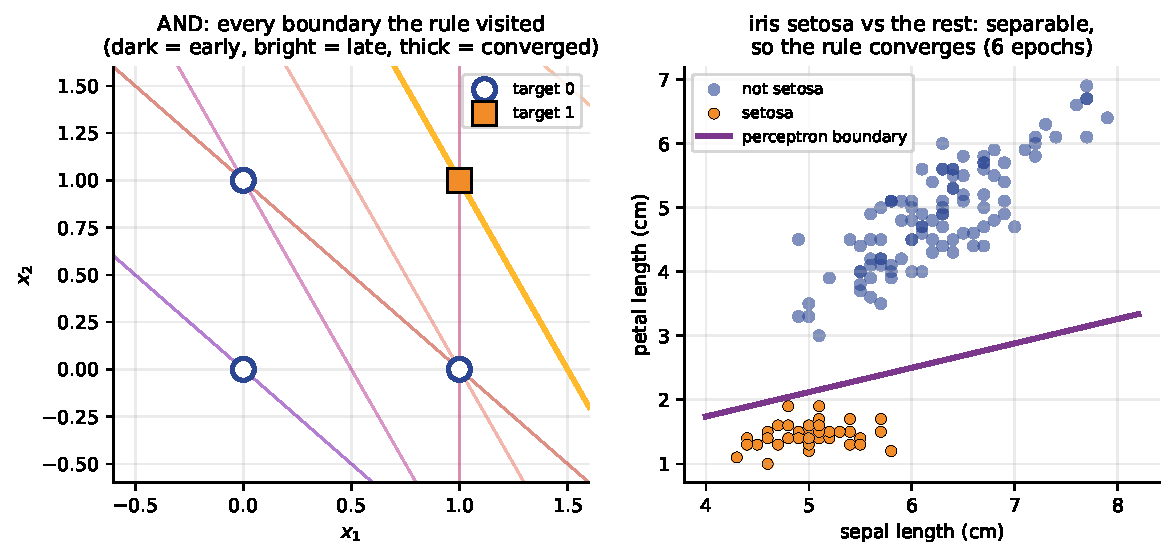
\includegraphics[width=0.98\textwidth]{perceptron.pdf}
  \caption{Left: the twelve weight states the rule visits on AND, dark early
    and bright late; the thick orange line is the converged rule
    $2x_1 + x_2 - 3 = 0$. Right: the same rule on \texttt{load\_iris}, setosa
    against the other two species --- linearly separable, so it converges, in
    six epochs again.}
  \label{fig:perceptron}
\end{figure}

\subsection{The same rule in code, on a real dataset}

Eight lines is the whole algorithm.

\begin{lstlisting}
def perceptron_fit(X, y, epochs=100, eta=1.0):
    w, b = np.zeros(X.shape[1]), 0.0
    for ep in range(epochs):
        errors = 0
        for k in range(len(X)):
            yh = 1.0 if (w @ X[k] + b) >= 0 else 0.0
            err = y[k] - yh
            if err != 0:
                w, b, errors = w + eta*err*X[k], b + eta*err, errors + 1
        if errors == 0: return w, b, ep + 1
\end{lstlisting}
\begin{codeout}
iris setosa vs rest, 150 rows, 2 features
   epoch  1  updates  1  training accuracy 0.6667
   epoch  2  updates  3  training accuracy 0.6667
   epoch  3  updates  3  training accuracy 0.6667
   epoch  4  updates  2  training accuracy 0.6667
   epoch  5  updates  1  training accuracy 1.0000
   epoch  6  updates  0  training accuracy 1.0000
   ...
   converged in 6 epochs, final training accuracy 1.0000
   final weights w = [+3.50 -9.20]  b = +2.00
   sklearn Perceptron on the same data: accuracy 1.0000
\end{codeout}

Setosa is separable from the other two iris species by a straight line in two
of the four measurements, so the rule terminates --- again in six epochs,
which is a coincidence, not a law.
\texttt{sklearn.linear\_model.Perceptron} is the same rule with bookkeeping
around it, and it reaches the same $1.0000$.

Notice the accuracy column. It sits at $0.6667$ for four epochs and then jumps
to $1.0000$. $0.6667$ is $100/150$, which is what you get by predicting
``not setosa'' for everything. The rule spends most of its life doing nothing
useful and then, in one epoch, finishes.

\subsection{What the rule guarantees, and what it does not}

\begin{keyidea}[Perceptron convergence theorem]
If the two classes are \textbf{linearly separable}, the rule reaches zero
training errors after a finite number of updates, bounded by $(R/\gamma)^2$
where $R = \max_i \|x_i\|$ and $\gamma$ is the margin of the best separating
hyperplane. The bound does not depend on $\eta$, on the order in which rows
are presented, or on where you start.
\end{keyidea}

That is a strong guarantee and it is worth knowing what it does \emph{not}
say. If the classes are not linearly separable, the theorem says nothing --- and
neither does the algorithm. It does not converge. It does not warn you. It
does not return the best line it saw along the way. It \textbf{cycles
forever}.

\begin{caution}
There is no ``stop when the error stops improving'' anywhere in
equation~\eqref{eq:percrule}. If you run the rule for a thousand epochs on
non-separable data and report the weights you happen to be holding at the end,
you are reporting an arbitrary point on a cycle. This is not small print. It
is the subject of the next section.
\end{caution}

% =========================================================================
\section{XOR: the wall, and the way through}
\label{sec:xor}

\subsection{Four rows the perceptron cannot learn}

Change two labels. Four rows again: $(0,0)\to 0$, $(0,1)\to \mathbf{1}$,
$(1,0)\to \mathbf{1}$, $(1,1)\to 0$. Output $1$ when the two inputs
\emph{differ}. This is exclusive OR.

Before reading on, commit to two numbers. Run the perceptron rule for a
thousand epochs: what training accuracy does it end on? And --- a different
question --- what is the best accuracy that \emph{any} straight line can
achieve on these four rows?

\begin{lstlisting}
w, b = np.zeros(2), 0.0
for ep in range(1000):
    for k in range(4):
        yh = 1.0 if (w @ X_xor[k] + b) >= 0 else 0.0
        w, b = w + (y_xor[k]-yh)*X_xor[k], b + (y_xor[k]-yh)
\end{lstlisting}
\begin{codeout}
perceptron on XOR, 1000 epochs
   best accuracy ever reached      0.50
   accuracy after the last epoch   0.50
   distinct (w1, w2, b) states visited: 2 -- it cycles, it does not settle
   sklearn Perceptron, 10000 iterations: accuracy 0.50
   logistic regression (also a single linear unit): accuracy 0.50
   exhaustive search over 81^3 = 531441 lines: the best any line achieves
   on XOR is 0.75 (3 of 4 rows), e.g. w = (-4.0, -4.0), b = +4.0
   any straight line splits the square into two halves; the two 1s are
   diagonally opposite, so no half-plane contains both and neither 0.
\end{codeout}

There are \emph{two separate failures} in that output and it is worth keeping
them apart.

\textbf{Failure one: no line is good enough.} An exhaustive search over
$81^3 = 531\,441$ lines on a grid finds that the best any of them achieves is
$\mathbf{0.75}$ --- three rows of four. This is a fact about the problem, not
about the algorithm.

\textbf{Failure two: the rule does not even find that line.} It ends on
$\mathbf{0.50}$, having visited only \emph{two} distinct end-of-epoch states
for a thousand epochs. It is on a cycle of length two. And logistic
regression, which \emph{is} differentiable and \emph{does} minimise a proper
loss, also gets $0.50$ --- because it is still one linear unit.

\subsection{Why no line works}
\label{sec:xorproof}

Two proofs, and you should be able to give either one in an examination.

\textbf{The geometry, in one sentence.} A line cuts the plane into two
half-planes. The two positives sit at $(0,1)$ and $(1,0)$, which are
\textbf{diagonally opposite corners} of the unit square. Any half-plane (a
convex set) that contains both must also contain everything on the segment
joining them, including the midpoint $(0.5, 0.5)$ --- which is also the
midpoint of the segment joining the two negatives $(0,0)$ and $(1,1)$. So the
same half-plane must contain part of the negatives' territory too.

\begin{worked}[The algebra, in four inequalities]
Suppose weights $w_1, w_2$ and bias $b$ exist with
$w_1x_1 + w_2x_2 + b \ge 0$ exactly on the two positive rows. Substituting the
four inputs:
\[
  \begin{array}{lll}
    \text{(1)} & b < 0 & \text{from } (0,0) \to 0\\
    \text{(2)} & w_2 + b \ge 0 & \text{from } (0,1) \to 1\\
    \text{(3)} & w_1 + b \ge 0 & \text{from } (1,0) \to 1\\
    \text{(4)} & w_1 + w_2 + b < 0 & \text{from } (1,1) \to 0
  \end{array}
\]
Add (2) and (3): $w_1 + w_2 + 2b \ge 0$. Rearranged, $w_1 + w_2 \ge -2b$.
Substitute into (4): $-2b + b < 0$, that is $-b < 0$, that is
$\mathbf{b > 0}$. This contradicts (1). No such $w_1, w_2, b$ exist.
\ensuremath{\square}
\end{worked}

This one page, published by Minsky and Papert in 1969, stopped
neural-network funding for roughly a decade. It is a completely correct
result about a \emph{single} unit, and it was widely read as a result about
neural networks in general, which it is not.

\subsection{By hand: two hidden units solve it}
\label{sec:xorhand}

Nothing new needs to be invented. Build XOR out of three perceptrons, each of
which we already know how to write down.

\begin{worked}[XOR from OR, AND and NOT]
Let the first hidden unit compute $\mathrm{OR}$: weights $(1,1)$, bias
$-0.5$, so it fires whenever $x_1 + x_2 \ge 0.5$, that is whenever at least
one input is $1$.

Let the second hidden unit compute $\mathrm{AND}$: weights $(1,1)$, bias
$-1.5$, so it fires only when $x_1 + x_2 \ge 1.5$, that is when both are $1$.

Now observe that $\mathrm{XOR} = \mathrm{OR}$ \emph{and not} $\mathrm{AND}$.
That is itself a linear function of $(h_1, h_2)$: weights $(+1, -1)$, bias
$-0.5$, giving $h_1 - h_2 \ge 0.5$.

Check all four rows by hand. For $(1,1)$: $h_1 = 1$, $h_2 = 1$, so
$h_1 - h_2 - 0.5 = -0.5 < 0$ and the output is $0$. Correct. For $(0,1)$:
$h_1 = 1$, $h_2 = 0$, so $1 - 0 - 0.5 = +0.5 \ge 0$ and the output is $1$.
Correct.
\end{worked}

\begin{codeout}
 x1 x2 | h1=OR h2=AND | y_hat | target
  0  0  |   0     0    |   0   |   0
  0  1  |   1     0    |   1   |   1
  1  0  |   1     0    |   1   |   1
  1  1  |   1     1    |   0   |   0
accuracy 1.00 -- the hidden layer moved (0,1) and (1,0) to the same point
hidden representation of the four inputs:
   (0,0) -> (0,0)
   (0,1) -> (1,0)
   (1,0) -> (1,0)
   (1,1) -> (1,1)
(0,1) and (1,0) both land on (1,0): once there, ONE line separates them
\end{codeout}

\subsection{The hidden layer is a change of coordinates}

Read the second half of that output again. It is the most important idea in
the lecture after backpropagation itself.

In the \emph{input} plane, the two positives are diagonally opposite and no
line separates them from the two negatives. In the \emph{hidden} plane, they
are \textbf{the same point}, $(1,0)$. Only three distinct points survive:
$(0,0)$, $(1,0)$ and $(1,1)$, and the middle one is the only positive. One
line separates it from the other two easily.

\begin{keyidea}
A hidden layer does not classify. It \textbf{re-represents} --- it maps the
input into a new space chosen so that a linear model works \emph{there}. The
output layer of every network in this course is still just logistic (or
linear) regression. Everything underneath it is learning the features that
regression needed and nobody had.
\end{keyidea}

\begin{figure}[htbp]
  \centering
  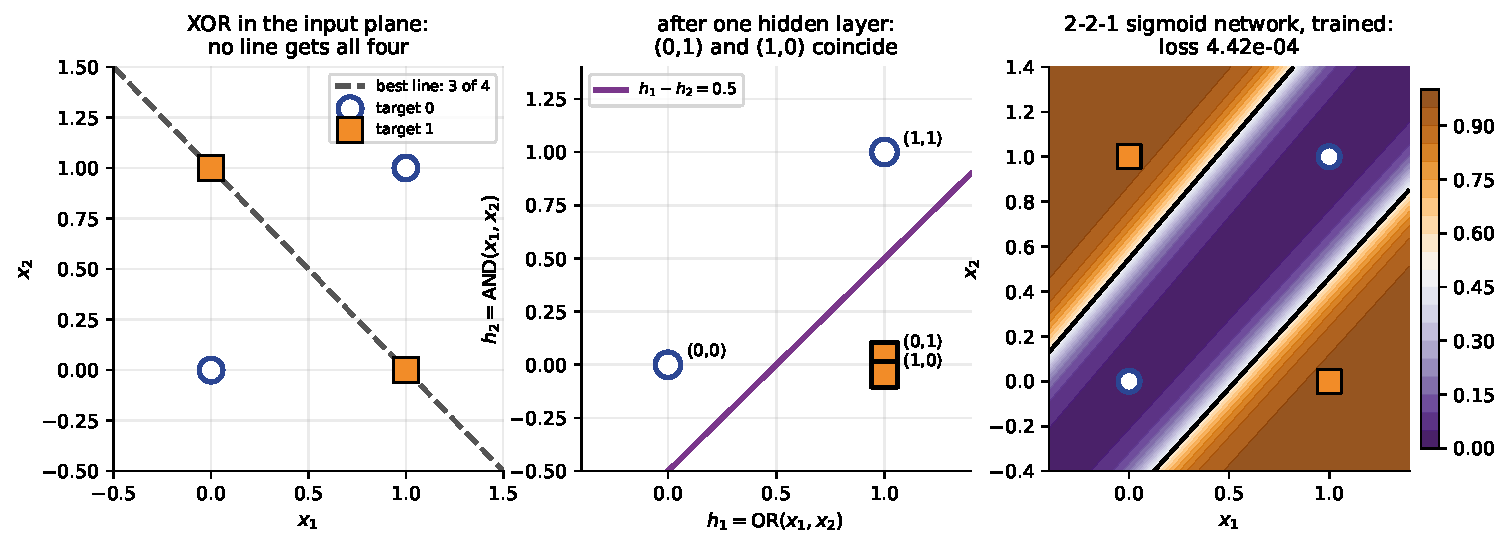
\includegraphics[width=0.98\textwidth]{xor.pdf}
  \caption{Left: the best straight line on XOR, three of four. Middle: after
    the hidden layer of Section~\ref{sec:xorhand}, the two positives coincide
    and a separating line does exist. Right: the decision surface of a trained
    $2$--$2$--$1$ sigmoid network, final loss $4.42\times10^{-4}$.}
  \label{fig:xor}
\end{figure}

\subsection{And the network finds those units for itself}

We chose OR and AND because we already knew them. A network trained by
gradient descent does not know them, and does not need to.

\begin{codeout}
2-2-1 sigmoid network trained on XOR, 20000 steps of full-batch descent
   loss at step     0: 0.125700
   loss at step  1000: 0.125008
   loss at step 20000: 0.000442
   outputs [0.0299 0.9717 0.9663 0.0265] against targets [0 1 1 0]
   accuracy 1.00
   learned hidden weights
      unit 1: w = [-5.80 +5.91]  b = +2.96
      unit 2: w = [-5.37 +5.17]  b = -2.81
   output layer: w = [-8.17 +8.66]  b = +3.80
   hidden units 1 -> final loss 0.118611
   hidden units 2 -> final loss 0.000442
   hidden units 3 -> final loss 0.000328
   hidden units 4 -> final loss 0.000397
   hidden units 8 -> final loss 0.000210
\end{codeout}

It did \emph{not} learn OR and AND. Unit 2 has weights $(-5.37, +5.17)$ and
bias $-2.81$, so it fires on ``$x_2$ and not $x_1$'' --- one of the two
detectors we built by hand. Unit 1 has weights $(-5.80, +5.91)$ and bias
$+2.96$, which fires \emph{everywhere except} at $(1,0)$; the output layer
gives it a strongly \textbf{negative} weight, $-8.17$, so what reaches the
output is its complement, ``$x_1$ and not $x_2$'' --- the other detector,
implemented upside down. The output then ORs the two, with the bias $+3.80$
holding the sum positive whenever unit 1 is off. That is the same
decomposition of XOR as ours with one half inverted, and there is no reason to
prefer either.

Read the last five lines as a capacity experiment. With \textbf{one} hidden
unit the loss stalls at $0.1186$, barely below the $0.1257$ it started at: one
hidden sigmoid unit leaves the whole network a monotone function of a single
linear score, so it can separate at most three of the four rows. With two it
reaches $4.42\times10^{-4}$. Beyond two the numbers wander between
$0.000210$ and $0.000397$ without a trend --- that is the initialisation
talking, not capacity. Two hidden units are what XOR needs, and the arithmetic
of Section~\ref{sec:xorhand} told us that before we ran anything.

\subsection{The feedforward network, in general}

Generalise. Write $a^{(0)} = x$ for the input, and for each layer
$\ell = 1, \dots, L$:
\begin{equation}
  z^{(\ell)} = W^{(\ell)\top} a^{(\ell-1)} + b^{(\ell)},
  \qquad
  a^{(\ell)} = \varphi^{(\ell)}\!\left(z^{(\ell)}\right).
  \label{eq:forward}
\end{equation}

Three pieces of vocabulary, all of which the examination uses:

\begin{itemize}[leftmargin=*]
  \item \textbf{Feedforward} --- the computation graph has no cycles.
    Information travels from input to output once. (Section~\ref{sec:rnn}
    breaks this.)
  \item \textbf{Fully connected}, or \textbf{dense} --- every unit in layer
    $\ell$ reads every unit in layer $\ell - 1$.
  \item \textbf{Multi-layer perceptron (MLP)} --- a feedforward, fully
    connected network with at least one hidden layer and a
    \emph{differentiable} activation.
\end{itemize}

\begin{caution}[An MLP is not made of perceptrons]
The name is historical and actively misleading. A perceptron has a step
activation; an MLP must \emph{not}, because backpropagation needs a
derivative and the step function's is zero almost everywhere. When you
describe a hidden layer, say ``unit'' or ``neuron'', not ``perceptron''.
\end{caution}

\begin{worked}[Counting parameters]
A layer from $n_{\text{in}}$ units to $n_{\text{out}}$ units has an
$n_{\text{in}} \times n_{\text{out}}$ weight matrix and an
$n_{\text{out}}$-vector of biases: $n_{\text{in}}n_{\text{out}} +
n_{\text{out}}$ parameters.

For the $64$--$32$--$10$ network of Section~\ref{sec:mlp}:
\[
  \underbrace{64 \cdot 32}_{2048} + \underbrace{32}_{\text{bias}}
  + \underbrace{32 \cdot 10}_{320} + \underbrace{10}_{\text{bias}}
  = \mathbf{2410}.
\]
Do this count every time you state an architecture. It is a one-mark question
that students routinely lose by forgetting the biases.
\end{worked}

% =========================================================================
\section{Activation functions, and why they are not optional}
\label{sec:act}

\subsection{Take the activation away and the network collapses}
\label{sec:collapse}

Suppose you build three layers and forget the non-linearity, so that
$\varphi$ is the identity everywhere. Then
\begin{align}
  f(x) &= \big((x W_1 + b_1)W_2 + b_2\big)W_3 + b_3 \notag\\
       &= x\,\underbrace{W_1W_2W_3}_{W_{\text{eff}}}
        + \underbrace{b_1W_2W_3 + b_2W_3 + b_3}_{b_{\text{eff}}}.
  \label{eq:collapse}
\end{align}

The proof is one line of algebra: a product of matrices is a matrix, a
composition of affine maps is an affine map. \textbf{Depth without
non-linearity buys nothing at all.} Whatever the three-layer network can
compute, the single affine map $x \mapsto xW_{\text{eff}} + b_{\text{eff}}$
computes too --- exactly, not approximately.

And there is a second, sharper consequence that is easy to miss. Rank is
subadditive under multiplication:
\[
  \operatorname{rank}(W_1W_2W_3)
  \le \min\big(\operatorname{rank} W_1, \operatorname{rank} W_2,
  \operatorname{rank} W_3\big).
\]
For a $4 \to 6 \to 5 \to 2$ stack, $W_{\text{eff}}$ is $4 \times 2$ and its
rank is at most $\min(4,6,5,2) = 2$. \textbf{A narrow layer caps what the
whole stack can express}, however wide the rest of it is --- and this bound
survives even when the activations are put back, in a weaker form.

\begin{lstlisting}
deep  = ((X @ W1 + b1) @ W2 + b2) @ W3 + b3
W_eff = W1 @ W2 @ W3
b_eff = b1 @ W2 @ W3 + b2 @ W3 + b3
flat  = X @ W_eff + b_eff
print(np.abs(deep - flat).max())
\end{lstlisting}
\begin{codeout}
three linear layers 4->6->5->2, no activation
   parameters in the deep version : 77
   parameters in the flat version : 10
   max |deep(x) - flat(x)| over 7 inputs: 7.105e-15
   W_eff = W1 W2 W3 has shape (4, 2) and rank 2
moons, 400 points
   logistic regression (1 linear unit)      accuracy 0.8750
   MLP 32-32 with identity activation       accuracy 0.8775
   MLP 32-32 with relu activation           accuracy 0.9625
   1058 parameters bought the identity network +0.0025 over 3 parameters
\end{codeout}

$7.105\times10^{-15}$ is floating-point noise at \texttt{float64}: the two
functions are the same function. Seventy-seven parameters were spent to
express something ten parameters express exactly.

The second half of the output is the same point on real data. On
\texttt{make\_moons} with 400 points, a $32$--$32$ MLP with \texttt{identity}
activation has $1058$ parameters and scores $0.8775$; plain logistic
regression has $3$ and scores $0.8750$. \textbf{A thousand parameters bought
$0.0025$}, which on 400 points is one row, and is noise. Change one string
--- \texttt{identity} to \texttt{relu} --- and the same architecture on the same
data with the same optimiser scores $0.9625$.

\begin{figure}[htbp]
  \centering
  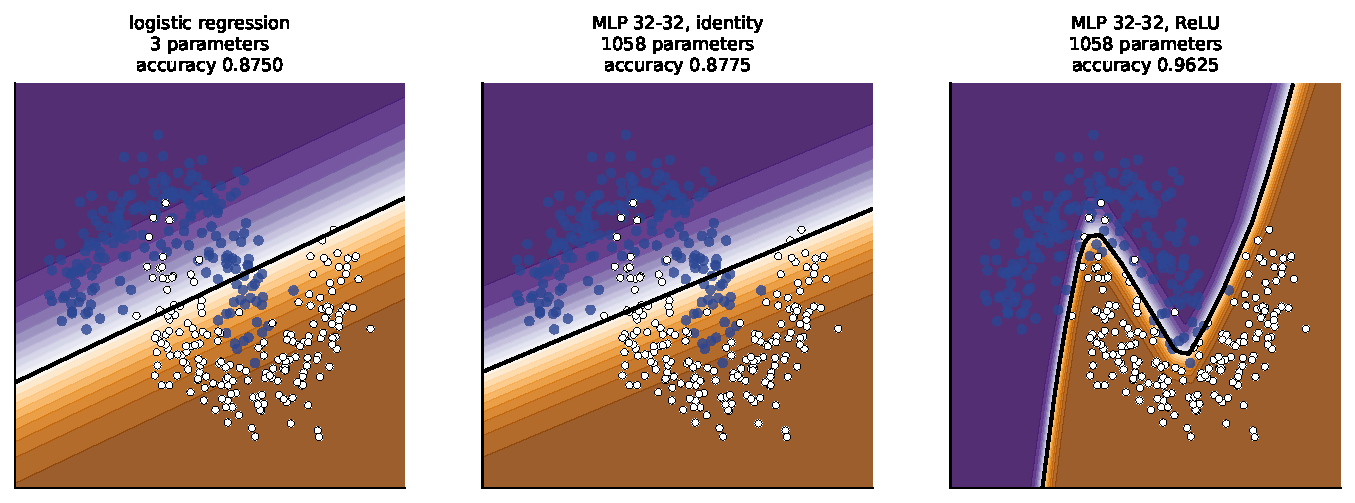
\includegraphics[width=0.94\textwidth]{linear.pdf}
  \caption{Same architecture, same data, same optimiser. The middle panel has
    $1058$ parameters and draws a straight line, because a straight line is
    all it can draw. Only the activation differs between the middle and right
    panels.}
  \label{fig:linear}
\end{figure}

\begin{keyidea}
The non-linearity is not a detail of the design and it is not there to
``add expressiveness'' vaguely. It is the only thing standing between your
deep network and a single matrix.
\end{keyidea}

\subsection{The three activations, and the derivatives backprop needs}
\label{sec:acts}

You need each function \emph{and} its derivative, because the derivative is
what the backward pass multiplies by.
\begin{align}
  \sigma(z) &= \frac{1}{1+e^{-z}},
    & \sigma'(z) &= \sigma(z)\big(1 - \sigma(z)\big)
    \label{eq:sig}\\
  \tanh z &= \frac{e^{z}-e^{-z}}{e^{z}+e^{-z}},
    & \tanh' z &= 1 - \tanh^2 z
    \label{eq:tanh}\\
  \mathrm{ReLU}(z) &= \max(0, z),
    & \mathrm{ReLU}'(z) &= \mathbf{1}[z > 0]
    \label{eq:relu}
\end{align}

Notice what the first two have in common: the derivative is expressible
\emph{in terms of the output}. If you have already computed $a = \sigma(z)$,
then $\sigma'(z) = a(1-a)$ costs one multiplication and one subtraction and
does not need $z$ at all. This is why an implementation of backpropagation
caches $a$, not $z$, for sigmoid and tanh layers. ReLU is the exception: it
needs the sign of $z$, which is why the NumPy code in
Section~\ref{sec:mlpcode} keeps the $z$ list.

\begin{worked}[$\sigma'(0)$ by hand]
$\sigma(0) = 1/(1 + e^{0}) = 1/2$ exactly. So
$\sigma'(0) = \tfrac12 \cdot \tfrac12 = \tfrac14$ exactly.

Is $1/4$ the maximum? Write $s = \sigma(z)$, so $\sigma' = s(1-s)$ with
$s \in (0,1)$. The parabola $s(1-s)$ has its vertex at $s = 1/2$ with value
$1/4$, and $s = 1/2$ happens exactly at $z = 0$. So
$\boxed{\sigma'(z) \le 1/4 \text{ for all } z}$, with equality only at the
origin. That single inequality drives the whole of
Section~\ref{sec:vanish}.
\end{worked}

\begin{codeout}
   z      sigmoid  s'(z)     tanh    t'(z)    relu   r'(z)
 -3.0    0.0474  0.0452  -0.9951  0.0099     0.0      0
 -1.0    0.2689  0.1966  -0.7616  0.4200     0.0      0
 -0.5    0.3775  0.2350  -0.4621  0.7864     0.0      0
 +0.0    0.5000  0.2500  +0.0000  1.0000     0.0      0
 +0.5    0.6225  0.2350  +0.4621  0.7864     0.5      1
 +1.0    0.7311  0.1966  +0.7616  0.4200     1.0      1
 +3.0    0.9526  0.0452  +0.9951  0.0099     3.0      1
max of sigmoid'  0.250000 at z = +0.0000   (exactly 1/4 at z = 0)
max of tanh'     1.000000 at z = +0.0000   (exactly 1 at z = 0)
sigmoid'(z) < 0.01 whenever |z| > 4.5849
0.25**10 = 9.536743e-07     1.0**10 = 1.0
\end{codeout}

Three numbers to memorise from that table. $\sigma'$ never exceeds
$\mathbf{0.25}$. $\tanh'$ never exceeds $\mathbf{1}$. $\mathrm{ReLU}'$ is
$\mathbf{1}$ or $\mathbf{0}$ --- it is a \emph{gate}, not a \emph{scale}: it
either passes the gradient through untouched or blocks it entirely, and it
never shrinks it.

The line $\sigma'(z) < 0.01$ whenever $|z| > 4.5849$ is worth a moment. A unit
whose pre-activation drifts beyond about $\pm 4.6$ is \textbf{saturated}: its
output is stuck near $0$ or $1$ and it passes less than one hundredth of the
gradient it receives. It has effectively stopped learning while still looking
perfectly healthy in the forward pass.

\begin{figure}[htbp]
  \centering
  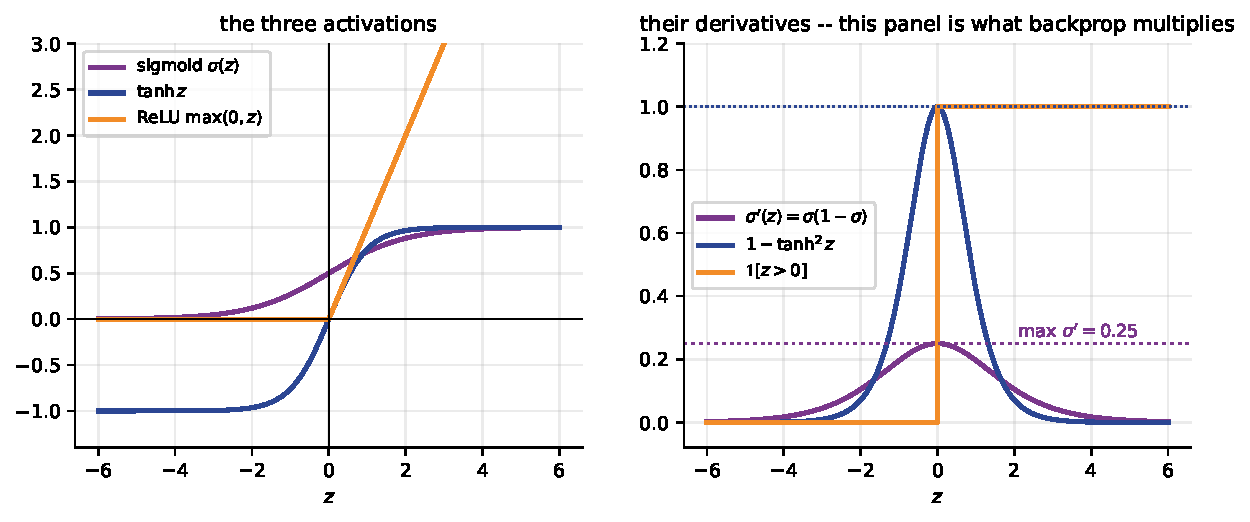
\includegraphics[width=0.82\textwidth]{activations.pdf}
  \caption{Left: what the forward pass computes. \textbf{Right: what the
    backward pass multiplies by}, once per layer. The dotted line on the right
    panel is at $0.25$.}
  \label{fig:activations}
\end{figure}

\subsection{Ten sigmoid layers, measured}
\label{sec:vanish}

Here is the experiment that turns $\sigma' \le 0.25$ into a number you will
remember. Build two networks of ten layers, sixteen units wide, with
\textbf{identical weights}. The only difference is the activation: one uses
sigmoid throughout, the other ReLU. Push the same batch through both, take the
same loss, and measure $\|\partial L / \partial W^{(1)}\|$ --- the size of the
gradient arriving at the layer nearest the input.

Commit to an order of magnitude before you look.

\begin{codeout}
ten layers of width 16, identical weights, only the activation differs
  layer   ||dL/dW|| sigmoid   ||dL/dW|| relu      ratio relu/sigmoid
    1        6.9609e-07         1.9017e-02           27320.0
    2        4.5222e-06         2.4150e-02            5340.4
    3        1.8296e-05         1.8996e-02            1038.2
    4        1.0142e-04         1.9325e-02             190.5
    5        3.3209e-04         1.4784e-02              44.5
    6        1.6433e-03         1.9475e-02              11.9
    7        8.5155e-03         2.2582e-02               2.7
    8        3.7576e-02         2.1301e-02               0.6
    9        1.3257e-01         3.3978e-02               0.3
   10        8.3697e-01         2.8907e-02               0.0
first-layer gradient norm, sigmoid : 6.9609e-07
first-layer gradient norm, relu    : 1.9017e-02
ratio (relu / sigmoid)             : 27320.0 x
attenuation across the sigmoid stack, layer 10 -> layer 1: 8.3167e-07
attenuation across the relu    stack, layer 10 -> layer 1: 6.5787e-01
for comparison, 0.25**9 = 3.8147e-06 and 0.25**10 = 9.5367e-07
\end{codeout}

The ratio at layer 1 is $\mathbf{27\,320}$, and it is not a mystery. Each
backward step through a sigmoid layer multiplies by $\sigma'(z) \le 0.25$; ten
of them multiply by at most $0.25^{10} = 9.54\times10^{-7}$, and the measured
attenuation from layer 10 down to layer 1 was $8.32\times10^{-7}$. \textbf{The
arithmetic predicted the measurement before the measurement was taken.}

Read the sigmoid column upwards and you can watch it happen: it falls by
roughly a factor of three to six \emph{per layer}, compounding. The ReLU
column is essentially flat --- it ends at $0.658$ of where it started, not at
$10^{-7}$.

The most instructive row is the last one. At layer 10, the sigmoid gradient is
$0.8370$ and the ReLU gradient is $0.0289$: the sigmoid network's gradient is
nearly thirty times the \emph{larger} of the two. The damage is not in the loss and not in the
top layer. It is \textbf{entirely in the propagation}.

\begin{figure}[htbp]
  \centering
  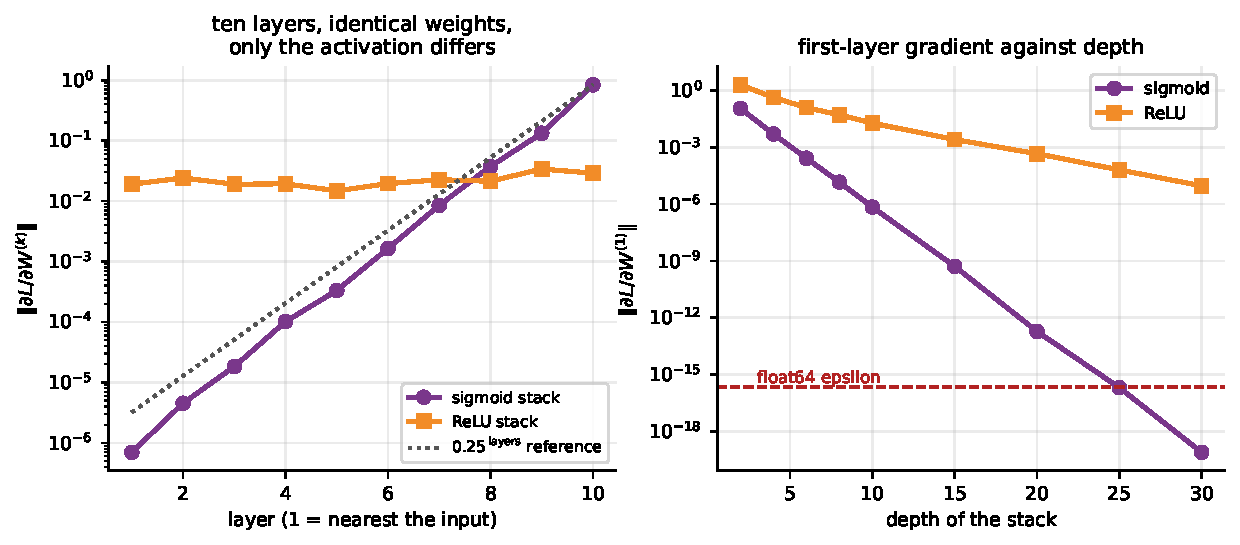
\includegraphics[width=0.80\textwidth]{vanishing.pdf}
  \caption{Depth against the surviving first-layer gradient, log axis. A
    straight line on a log axis is geometric decay.}
  \label{fig:vanishing}
\end{figure}

\begin{codeout}
   depth  2  sigmoid layer-1 norm 1.129e-01   relu layer-1 norm 2.009e+00
   depth  5  sigmoid layer-1 norm 1.125e-03   relu layer-1 norm 1.541e-01
   depth 10  sigmoid layer-1 norm 6.961e-07   relu layer-1 norm 1.902e-02
   depth 20  sigmoid layer-1 norm 1.875e-13   relu layer-1 norm 4.608e-04
   depth 30  sigmoid layer-1 norm 7.569e-20   relu layer-1 norm 9.209e-06
\end{codeout}

Thirty sigmoid layers put the first-layer gradient at $7.6\times10^{-20}$.
Against a weight of order one, in single precision --- where the spacing
between representable numbers near $1$ is about $1.2\times10^{-7}$ --- that
update is not small, it is \emph{nothing}. The weight does not move.

\subsection{And this is not a thought experiment}

The same comparison, on real data, with a real classifier.

\begin{codeout}
30 epochs, learning rate 0.1, hidden layers of 32 units each
  activation  hidden layers   train loss   test accuracy
   relu            1           0.0758        0.9711
   relu            3           0.0114        0.9733
   relu            6           0.0030        0.9667
   relu           10           0.2811        0.8778
   sigmoid         1           0.3303        0.9422
   sigmoid         3           2.3062        0.1000
   sigmoid         6           2.3227        0.1000
   sigmoid        10           2.3184        0.1000
chance is 0.1000. A sigmoid network of 3 hidden layers does not train
at all here: the gradient reaching layer 1 is too small to move it.
\end{codeout}

Chance on ten balanced classes is $0.1000$, and a cross-entropy loss of
$\ln 10 = 2.3026$ is exactly the loss of a network that outputs a uniform
distribution over the ten classes regardless of input. Look at the sigmoid
rows: $2.3062$, $2.3227$, $2.3184$. \textbf{Three sigmoid hidden layers do
not train badly. They do not train at all.} The network is still emitting its
initial uniform guess after thirty epochs.

ReLU is fine to six hidden layers and starts to strain at ten
($0.8778$, and a training loss that went \emph{up}). That is an honest
result and it is the reason residual connections were invented --- but
residual connections are a Unit VII topic and $0.9733$ at three layers is
what this course needs.

\begin{caution}[Sigmoid still has a place]
None of this says sigmoid is wrong. It is the correct \emph{output} activation
for binary classification, because you want a probability, and there is only
one output layer so nothing compounds. What it is bad at is being a
\emph{hidden} activation in a deep stack. Use ReLU (or tanh) in the hidden
layers and sigmoid or softmax at the top.
\end{caution}

% =========================================================================
\section{Backpropagation, derived in full}
\label{sec:bp}

\subsection{Backpropagation is the chain rule, and nothing else}

For a composition $x \to h_1 \to h_2 \to y \to L$, the chain rule says
\begin{equation}
  \frac{\partial L}{\partial x}
  = \frac{\partial L}{\partial y}\,
    \frac{\partial y}{\partial h_2}\,
    \frac{\partial h_2}{\partial h_1}\,
    \frac{\partial h_1}{\partial x}.
  \label{eq:chain}
\end{equation}

That is not new and it is not the interesting part. The interesting part is
that matrix products are associative, so you may evaluate
equation~\eqref{eq:chain} in either order --- and the two orders cost wildly
different amounts.

Evaluate it \textbf{right to left}, starting from $\partial h_1/\partial x$,
and you are propagating derivatives \emph{forwards}. You need one pass per
input variable: a million parameters means a million passes. This is called
\emph{forward-mode} differentiation, and it is the right choice when there are
few inputs and many outputs.

Evaluate it \textbf{left to right}, starting from the single scalar $L$, and
one pass covers every parameter at once. This is \emph{reverse-mode}
differentiation, and in a neural network --- millions of inputs, one scalar
output --- it is the only one that is affordable. \textbf{Reverse-mode
differentiation applied to a layered network is what we call
backpropagation.}

\begin{keyidea}
One forward pass and one backward pass give you the derivative of the loss
with respect to \emph{every} parameter, at a cost of roughly twice the forward
pass. Not once per parameter. That asymmetry is the entire reason deep
learning is computationally possible.
\end{keyidea}

The second structural idea is \textbf{locality}. Each layer is handed
$\partial L / \partial(\text{its output})$ and must return two things:
$\partial L / \partial(\text{its input})$, to pass further down, and
$\partial L / \partial(\text{its parameters})$, to keep. It supplies only its
\emph{own} derivative and multiplies through. It does not know what is above
it or below it. That is why you can write a layer once, test it once, and
compose it forever --- and it is the design of every autodiff library
including \texttt{gradkit}.

\subsection{The network we are going to differentiate}
\label{sec:tinynet}

Two inputs, two hidden units, one output, sigmoid everywhere, squared-error
loss. Nine parameters --- small enough to do entirely with a pen, large enough
that every case appears: two layers, a shared downstream path, and biases.

\textbf{Copy these numbers down.}

\begin{center}
\begin{tabular}{llll}
  \toprule
  \multicolumn{4}{l}{\textbf{Inputs and target}}\\
  $x_1$ & $1.0$ & $x_2$ & $2.0$ \\
  $t$ & $1.0$ & &\\
  \midrule
  \multicolumn{4}{l}{\textbf{Input-to-hidden weights and biases}}\\
  $w_{11}$ & $+0.2$ & $w_{12}$ & $+0.3$\\
  $w_{21}$ & $-0.1$ & $w_{22}$ & $+0.1$\\
  $b_{11}$ & $\phantom{+}0.0$ & $b_{12}$ & $+0.5$\\
  \midrule
  \multicolumn{4}{l}{\textbf{Hidden-to-output weights and bias}}\\
  $v_1$ & $+0.4$ & $v_2$ & $-0.6$\\
  $b_2$ & $+0.1$ & &\\
  \bottomrule
\end{tabular}
\end{center}

The forward equations, in full, with the index convention $w_{ij}$ = weight
from input $i$ to hidden unit $j$:
\begin{align}
  z_1 &= w_{11}x_1 + w_{21}x_2 + b_{11}, & a_1 &= \sigma(z_1)
    \label{eq:tf1}\\
  z_2 &= w_{12}x_1 + w_{22}x_2 + b_{12}, & a_2 &= \sigma(z_2)
    \label{eq:tf2}\\
  z_3 &= v_1a_1 + v_2a_2 + b_2,          & a_3 &= \sigma(z_3)
    \label{eq:tf3}\\
  L   &= \tfrac{1}{2}(a_3 - t)^2. & &
    \label{eq:tloss}
\end{align}

The factor of $\tfrac12$ in the loss is there only so that the $2$ from
differentiating the square cancels. It changes no gradient's sign and no
argument.

\subsection{Forward pass, by hand}
\label{sec:fwd}

\begin{worked}[Every number of the forward pass]
\textbf{Hidden unit 1.}
\[
  z_1 = (0.2)(1.0) + (-0.1)(2.0) + 0.0 = 0.2 - 0.2 + 0.0 = 0.0,
\]
so $a_1 = \sigma(0) = \mathbf{0.5000000000}$ exactly. The weights were chosen
to make this happen: $\sigma(0) = 1/2$ and $\sigma'(0) = 1/4$ are both exact,
so the hidden-layer arithmetic below can be checked without a calculator.

\textbf{Hidden unit 2.}
\[
  z_2 = (0.3)(1.0) + (0.1)(2.0) + 0.5 = 0.3 + 0.2 + 0.5 = 1.0,
\]
so $a_2 = \sigma(1) = 1/(1+e^{-1}) = \mathbf{0.7310585786}$.

\textbf{Output unit.}
\[
  z_3 = (0.4)(0.5000000000) + (-0.6)(0.7310585786) + 0.1
      = 0.2 - 0.4386351472 + 0.1 = \mathbf{-0.1386351472},
\]
so $a_3 = \sigma(-0.1386351472) = \mathbf{0.4653966177}$.

\textbf{Loss.}
\[
  L = \tfrac12(0.4653966177 - 1.0)^2
    = \tfrac12(-0.5346033823)^2
    = \tfrac12(0.2858007764) = \mathbf{0.1429003882}.
\]
\end{worked}

\begin{codeout}
inputs   x1 = 1.0   x2 = 2.0      target t = 1.0
weights  w11 +0.2  w12 +0.3  w21 -0.1  w22 +0.1  b11 +0.0  b12 +0.5
         v1  +0.4  v2  -0.6  b2  +0.1
z1 = 0.2*1.0 + -0.1*2.0 + 0.0 = +0.0000   a1 = sigma(z1) = 0.5000000000
z2 = 0.3*1.0 + 0.1*2.0 + 0.5 = +1.0000   a2 = sigma(z2) = 0.7310585786
z3 = 0.4*0.5000000000 + -0.6*0.7310585786 + 0.1 = -0.1386351472
a3 = sigma(z3) = 0.4653966177
L  = 0.5 * (0.4653966177 - 1.0)^2 = 0.1429003882
\end{codeout}

\begin{figure}[htbp]
  \centering
  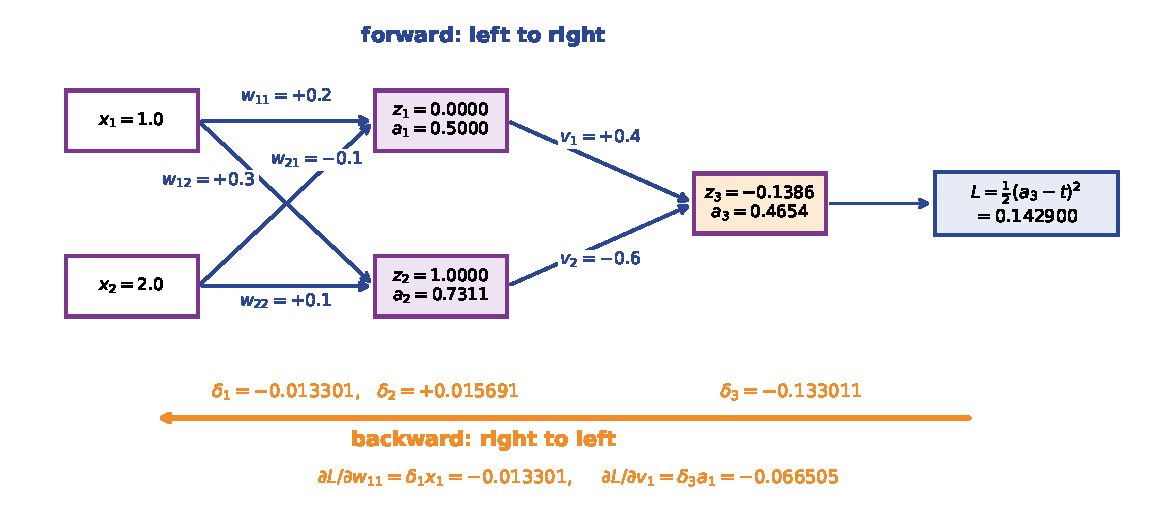
\includegraphics[width=0.86\textwidth]{tinynet.pdf}
  \caption{The nine-parameter network of Section~\ref{sec:tinynet}, forward
    and backward. Every number on this figure was produced by the code, not
    typed onto it. The orange arrow is the direction of the next four
    subsections.}
  \label{fig:tinynet}
\end{figure}

\subsection{Backward, step 1: the output unit}

Define $\delta_3 = \partial L / \partial z_3$. It factors into two pieces by
the chain rule, and both are one line.

\begin{worked}[$\delta_3$]
\textbf{The loss derivative.} $L = \tfrac12(a_3 - t)^2$, so
\[
  \frac{\partial L}{\partial a_3} = a_3 - t
  = 0.4653966177 - 1.0 = \mathbf{-0.5346033823}.
\]
It is negative because the output is \emph{below} the target: increasing
$a_3$ would decrease the loss.

\textbf{The activation derivative.} By equation~\eqref{eq:sig},
\[
  \frac{\partial a_3}{\partial z_3} = a_3(1 - a_3)
  = (0.4653966177)(0.5346033823) = \mathbf{+0.2488026059}.
\]
Sanity check: it must be positive and at most $0.25$, and $0.2488$ is just
under $0.25$ because $a_3$ is close to $0.5$.

\textbf{The product.}
\[
  \delta_3 = \frac{\partial L}{\partial z_3}
  = \frac{\partial L}{\partial a_3}\cdot\frac{\partial a_3}{\partial z_3}
  = (-0.5346033823)(0.2488026059) = \mathbf{-0.1330107147}.
\]
\end{worked}

$\delta_3$ is the whole of the output layer's message to everything below it.
\textbf{One number.} Every gradient in this network is $\delta_3$ multiplied
by something local.

\subsection{Backward, step 2: the output layer's own weights}

Because $z_3 = v_1a_1 + v_2a_2 + b_2$, we have $\partial z_3/\partial v_1 =
a_1$, $\partial z_3/\partial v_2 = a_2$ and $\partial z_3/\partial b_2 = 1$.
Multiply each by $\delta_3$:
\begin{align}
  \frac{\partial L}{\partial v_1}
    &= \delta_3 a_1 = (-0.1330107147)(0.5000000000)
     = \mathbf{-0.0665053573}\\
  \frac{\partial L}{\partial v_2}
    &= \delta_3 a_2 = (-0.1330107147)(0.7310585786)
     = \mathbf{-0.0972386240}\\
  \frac{\partial L}{\partial b_2}
    &= \delta_3 \cdot 1 = \mathbf{-0.1330107147}
\end{align}

\begin{keyidea}
The pattern, already visible and true for every weight in every network:
\[
  \text{gradient of a weight} \;=\; \text{delta at its output end}
  \;\times\; \text{the activation at its input end}.
\]
A bias multiplies the constant $1$, so its gradient is the delta itself. That
is the whole rule for biases, at every layer, forever.
\end{keyidea}

\subsection{Backward, step 3: push the delta through the hidden layer}
\label{sec:recursion}

This is the line that puts the ``back'' in backpropagation. We want
$\delta_1 = \partial L / \partial z_1$. The only route from $z_1$ to $L$ goes
$z_1 \to a_1 \to z_3 \to L$, so
\[
  \delta_1
  = \underbrace{\frac{\partial L}{\partial z_3}}_{\delta_3}
    \cdot \underbrace{\frac{\partial z_3}{\partial a_1}}_{v_1}
    \cdot \underbrace{\frac{\partial a_1}{\partial z_1}}_{a_1(1-a_1)}.
\]

\begin{worked}[$\delta_1$ and $\delta_2$]
\[
  \delta_1 = (-0.1330107147)(0.4)\underbrace{(0.5)(0.5)}_{=\,0.25}
  = (-0.1330107147)(0.1) = \mathbf{-0.0133010715}.
\]
Note $a_1(1-a_1) = 0.25$ \emph{exactly}, because $a_1 = 0.5$ exactly. This
unit sits at the steepest point of the sigmoid: it is passing the most
gradient a sigmoid unit can ever pass, and it is still only a quarter.
\[
  \delta_2 = \delta_3 \cdot v_2 \cdot a_2(1-a_2)
  = (-0.1330107147)(-0.6)(0.7310585786)(0.2689414214)
  = \mathbf{+0.0156908963}.
\]
$\delta_2$ has the \emph{opposite sign} to $\delta_3$, because $v_2$ is
negative. And $a_2(1-a_2) = 0.1966$, well under $0.25$, because $a_2$ has
drifted away from $0.5$.
\end{worked}

Three things happened to the message on its way down. It was
\textbf{routed} along the weight it came down ($v_j$) --- so a unit that
contributes strongly to the output receives a strong correction. It was
\textbf{signed} by that weight. And it was \textbf{throttled} by the local
derivative $\sigma'$, which is at most $0.25$. Do that ten times and you have
Section~\ref{sec:vanish}.

\subsection{Backward, step 4: the input layer's weights}

Exactly the same rule as step 2, one layer down: delta times the activation at
the input end, which here is just the input itself.
\begin{align}
  \frac{\partial L}{\partial w_{11}} &= \delta_1 x_1
    = (-0.0133010715)(1.0) = \mathbf{-0.0133010715}\\
  \frac{\partial L}{\partial w_{21}} &= \delta_1 x_2
    = (-0.0133010715)(2.0) = \mathbf{-0.0266021429}\\
  \frac{\partial L}{\partial b_{11}} &= \delta_1
    = \mathbf{-0.0133010715}\\
  \frac{\partial L}{\partial w_{12}} &= \delta_2 x_1
    = (+0.0156908963)(1.0) = \mathbf{+0.0156908963}\\
  \frac{\partial L}{\partial w_{22}} &= \delta_2 x_2
    = (+0.0156908963)(2.0) = \mathbf{+0.0313817925}\\
  \frac{\partial L}{\partial b_{12}} &= \delta_2
    = \mathbf{+0.0156908963}
\end{align}

\begin{codeout}
dL/da3   = a3 - t                    = -0.5346033823
da3/dz3  = a3(1 - a3)                = +0.2488026059
delta3   = dL/dz3                    = -0.1330107147
dL/dv1   = delta3 * a1               = -0.0665053573
dL/dv2   = delta3 * a2               = -0.0972386240
dL/db2   = delta3                    = -0.1330107147
delta1   = delta3 * v1 * a1(1 - a1)  = -0.0133010715
delta2   = delta3 * v2 * a2(1 - a2)  = +0.0156908963
dL/dw11  = delta1 * x1               = -0.0133010715
dL/dw21  = delta1 * x2               = -0.0266021429
dL/db11  = delta1                    = -0.0133010715
dL/dw12  = delta2 * x1               = +0.0156908963
dL/dw22  = delta2 * x2               = +0.0313817925
dL/db12  = delta2                    = +0.0156908963
\end{codeout}

\begin{caution}[Why you scale your features]
$\partial L/\partial w_{21}$ is exactly \emph{twice}
$\partial L/\partial w_{11}$, and the only reason is that $x_2 = 2x_1$. An
input twice as large gets a gradient twice as large, and therefore takes a
step twice as large for the same learning rate. If one of your columns is in
rupees and another is a count between $0$ and $1$, the ratio is not two, it is
ten thousand, and no single learning rate is right for both. \textbf{Scale
your features before training a network} --- see Section~\ref{sec:scaling}
for the measurement.
\end{caution}

\subsection{The two rules, stated once, for any depth}
\label{sec:tworules}

Everything above generalises to $L$ layers of any width, and it fits on one
line each. Write $\odot$ for elementwise multiplication.
\begin{align}
  \delta^{(\ell)}
    &= \left(W^{(\ell+1)}\delta^{(\ell+1)}\right)
       \odot \varphi'\!\left(z^{(\ell)}\right)
    &&\text{\emph{propagate}}
    \label{eq:bp1}\\
  \frac{\partial L}{\partial W^{(\ell)}}
    &= a^{(\ell-1)}\delta^{(\ell)\top},
    \qquad
    \frac{\partial L}{\partial b^{(\ell)}} = \delta^{(\ell)}
    &&\text{\emph{read off}}
    \label{eq:bp2}
\end{align}
started at the top with
$\delta^{(L)} = \nabla_{a}L \odot \varphi'(z^{(L)})$.

\textbf{That is the entire algorithm.} Apply \eqref{eq:bp1} to walk down one
layer; apply \eqref{eq:bp2} at each layer to read off the gradients you came
for; stop when you reach the input.

\begin{caution}[Two shapes to get right]
First, the $\odot$ in \eqref{eq:bp1} is \textbf{elementwise}, not a matrix
product. The Jacobian of an elementwise activation is diagonal, and
multiplying by a diagonal matrix is elementwise multiplication by its
diagonal. Writing it as a matrix product is the commonest algebra error here.

Second, for a batch of $n$ rows, the \textbf{bias gradient is the sum over the
batch}, because the one bias vector was broadcast to all $n$ rows. In NumPy
that is \texttt{d.sum(0)}. Forgetting the sum --- or writing
\texttt{d.mean(0)} when the loss is already averaged elsewhere --- is the
single commonest bug in a hand-written backward pass, and it produces a
network that trains, slowly and wrongly.
\end{caution}

\subsection{Verified once: central finite differences}
\label{sec:gradcheck}

We now have nine numbers computed with a pen. Check them the dumb way. For
each parameter $p$, nudge it by $h$ in each direction, run the forward pass
twice, and take the central difference
\begin{equation}
  \frac{\partial L}{\partial p} \approx
  \frac{L(p + h) - L(p - h)}{2h}.
  \label{eq:fd}
\end{equation}

Before you look: with $h = 10^{-6}$, how closely should the two agree? Give
your answer as a power of ten.

\begin{lstlisting}
h = 1e-6
for k in base:                       # base = the nine parameters
    up, dn = dict(base), dict(base)
    up[k], dn[k] = base[k] + h, base[k] - h
    fd = (tiny_loss(up) - tiny_loss(dn)) / (2 * h)
    print(k, hand[k], fd, abs(fd - hand[k]))
\end{lstlisting}
\begin{codeout}
parameter   hand-computed      finite difference    |difference|
   w11      -0.013301071466     -0.013301071425     4.107e-11
   w12      +0.015690896251     +0.015690896291     4.005e-11
   w21      -0.026602142932     -0.026602142905     2.662e-11
   w22      +0.031381792501     +0.031381792540     3.846e-11
   b11      -0.013301071466     -0.013301071425     4.107e-11
   b12      +0.015690896251     +0.015690896291     4.005e-11
   v1       -0.066505357329     -0.066505357305     2.492e-11
   v2       -0.097238624001     -0.097238623986     1.502e-11
   b2       -0.133010714659     -0.133010714679     1.954e-11
largest disagreement over all nine parameters: 4.107e-11
that is the finite-difference truncation error, not a backprop error:
   the central difference is accurate to O(h^2) = O(1e-12)
\end{codeout}

Nine for nine, to ten significant figures. The largest disagreement is
$\mathbf{4.107\times10^{-11}}$, and that residue belongs to the \emph{finite
difference}, not to backpropagation. Taylor-expanding both terms of
equation~\eqref{eq:fd} shows the odd-order terms cancel and the leading error
is $\tfrac{h^2}{6}L'''(p) = O(10^{-12})$, degraded a little by catastrophic
cancellation when two nearly equal loss values are subtracted.

\begin{caution}[Use the central difference, and use \texttt{float64}]
The forward difference $(L(p+h)-L(p))/h$ is only $O(h)$ accurate and would
give you about $10^{-6}$ here --- five orders of magnitude worse for the same
work. And do not do any of this in \texttt{float32}: the subtraction in the
numerator loses most of its significant digits, and you will conclude your
correct gradient is wrong.
\end{caution}

\begin{tryit}[Gradient-check every backward pass you write]
Take any network you have written, freeze a batch, and run the loop above over
twenty randomly chosen weight entries. Expect agreement to about $10^{-10}$ in
\texttt{float64} with $h = 10^{-6}$. If you see $10^{-2}$, you have a bug. If
you see $2\times$ the right answer, you have forgotten a factor somewhere ---
and note that a gradient wrong by a constant factor \emph{still trains}, just
worse, so you will spend a week blaming the learning rate. Four lines of
checking now saves that week.
\end{tryit}

\subsection{Verified twice: autodiff, in a library you can open}
\label{sec:gradkit}

The second check uses \texttt{gradkit}, the course's from-scratch autodiff
library. It is not a black box: the point of using it here is that you can
open \texttt{src/gradkit/functions/activation.py} and find $\sigma(1-\sigma)$
written out exactly as we wrote it in Section~\ref{sec:acts}.

\begin{lstlisting}
import gradkit as gk
W1g = gk.tensor(W1, requires_grad=True); b1g = gk.tensor(b1, requires_grad=True)
W2g = gk.tensor(W2.reshape(2,1), requires_grad=True); b2g = gk.tensor([b2], requires_grad=True)
a1g = gk.sigmoid(gk.tensor(x.reshape(1,2)) @ W1g + b1g)
a2g = gk.sigmoid(a1g @ W2g + b2g)
Lg  = ((a2g - tg) * (a2g - tg)).sum() * 0.5
Lg.backward()
\end{lstlisting}
\begin{codeout}
gradkit forward loss  0.142900388188   (hand: 0.142900388188)
parameter    hand            gradkit          |difference|
   w11    -0.013301071466   -0.013301071466    0.000e+00
   w12    +0.015690896251   +0.015690896251    0.000e+00
   w21    -0.026602142932   -0.026602142932    0.000e+00
   w22    +0.031381792501   +0.031381792501    0.000e+00
   b11    -0.013301071466   -0.013301071466    0.000e+00
   b12    +0.015690896251   +0.015690896251    0.000e+00
   v1     -0.066505357329   -0.066505357329    0.000e+00
   v2     -0.097238624001   -0.097238624001    0.000e+00
   b2     -0.133010714659   -0.133010714659    0.000e+00
largest hand-vs-autodiff disagreement: 0.000e+00
largest hand-vs-finite-difference disagreement: 4.107e-11
all nine hand-computed gradients confirmed twice
\end{codeout}

\textbf{Zero}, bit for bit. Not ``very small'' --- exactly zero. That is worth
pausing on, because it is the strongest evidence available that
backpropagation is not an approximation. Automatic differentiation evaluates
the same product of the same local derivatives in the same order, using the
same floating-point operations, so it produces the same bits.

\begin{keyidea}
Finite differences agree to $4\times10^{-11}$ because they are an
\emph{approximation} of the derivative. Autodiff agrees to $0$ because it
\emph{is} the derivative, computed by the rules you just applied by hand. A
library does not know a better chain rule than you do.
\end{keyidea}

\subsection{What you do with nine gradients}

Descend. $p \leftarrow p - \eta\,\partial L/\partial p$, for all nine at once.

\begin{codeout}
   eta   0.5   loss 0.1429003882 -> 0.1263134462   (-1.66e-02)
   eta   5.0   loss 0.1429003882 -> 0.0297255097   (-1.13e-01)
   eta  50.0   loss 0.1429003882 -> 0.0000000004   (-1.43e-01)
   after   1 steps at eta=5.0: loss 0.02972551  output 0.756174
   after  10 steps at eta=5.0: loss 0.00262249  output 0.927578
   after 100 steps at eta=5.0: loss 0.00021488  output 0.979270
   after 500 steps at eta=5.0: loss 0.00003898  output 0.991170
\end{codeout}

The output climbs $0.4654 \to 0.7562 \to 0.9276 \to 0.9793 \to 0.9912$ towards
its target of $1.0$, and the loss falls monotonically. That is the whole
training loop, on one row.

\begin{caution}
Do not read anything into $\eta = 50$ working here. This is \emph{one}
training row, and one row can always be fitted --- the loss surface in that
direction is a simple bowl with nothing to overshoot into. On a real dataset
with a thousand rows pulling in different directions, $\eta = 50$ diverges on
the first mini-batch.
\end{caution}

\subsection{One special case worth memorising: softmax with cross-entropy}
\label{sec:softmax}

For classification you do not use squared error. You use a softmax output and
cross-entropy loss:
\[
  p_c = \frac{e^{z_c}}{\sum_{k} e^{z_k}},
  \qquad
  L = -\sum_c y_c \log p_c,
\]
with $y$ the one-hot target. Differentiating this looks unpleasant --- the
softmax Jacobian is $\partial p_i/\partial z_j = p_i(\delta_{ij} - p_j)$ ---
but the $1/p$ coming from the logarithm cancels it exactly, and the result is
as simple as it could possibly be:
\begin{equation}
  \frac{\partial L}{\partial z} = p - y.
  \label{eq:softmaxgrad}
\end{equation}

\begin{codeout}
logits z          = [2.0 1.0 0.1]
softmax p         = [0.659001 0.242433 0.098566]
target one-hot y  = [0 1 0]
L = -log p_1      = 1.417030
claim: dL/dz = p - y = [+0.659001 -0.757567 +0.098566]
finite difference    = [+0.659001 -0.757567 +0.098566]
largest disagreement = 2.168e-10
the softmax Jacobian and the log both cancel: that is why the output
layer of the digits network above needs no activation derivative at all.
\end{codeout}

So the output layer of a classifier needs \textbf{no activation derivative at
all} in code. The delta is one subtraction: \texttt{(probs - onehot)}. That is
why the NumPy network in the next section starts its backward pass with a
single line and no $\varphi'$ term.

% =========================================================================
\section{An MLP, from scratch, on real data}
\label{sec:mlp}

\subsection{The algorithm in eight lines}

For each mini-batch of $n$ rows:

\begin{enumerate}[leftmargin=*]
  \item $a^{(0)} \leftarrow X_{\text{batch}}$
  \item for $\ell = 1 \dots L$: \;
    $z^{(\ell)} = a^{(\ell-1)}W^{(\ell)} + b^{(\ell)}$, \;
    $a^{(\ell)} = \varphi(z^{(\ell)})$ \hfill \emph{forward}
  \item $\delta^{(L)} \leftarrow (a^{(L)} - Y)/n$
    \hfill \emph{softmax + cross-entropy, eq.~\eqref{eq:softmaxgrad}}
  \item for $\ell = L \dots 1$:
  \item \quad $\nabla W^{(\ell)} = a^{(\ell-1)\top}\delta^{(\ell)}$, \;
    $\nabla b^{(\ell)} = \sum_{\text{rows}} \delta^{(\ell)}$
    \hfill \emph{read off, eq.~\eqref{eq:bp2}}
  \item \quad $\delta^{(\ell-1)} =
    \big(\delta^{(\ell)}W^{(\ell)\top}\big)\odot\varphi'(z^{(\ell-1)})$
    \hfill \emph{propagate, eq.~\eqref{eq:bp1}}
  \item $W^{(\ell)} \leftarrow W^{(\ell)} - \eta\nabla W^{(\ell)}$ for every
    $\ell$ \hfill \emph{update}
  \item repeat over all batches; that is one \textbf{epoch}
\end{enumerate}

Lines 5 and 6 are the two rules of Section~\ref{sec:tworules}, in matrix form
with the batch dimension leading. Nothing has been added.

\subsection{Written out in NumPy}
\label{sec:mlpcode}

Fourteen lines, no framework.

\begin{lstlisting}
def forward(P, X):
    A, Z = [X], []
    for k, (W, b) in enumerate(P):
        z = A[-1] @ W + b; Z.append(z)
        A.append(softmax(z) if k == len(P)-1 else relu(z))
    return A, Z

def backward(P, A, Z, Y):
    n, grads = len(Y), [None] * len(P)
    d = (A[-1] - Y) / n                 # softmax + cross-entropy, combined
    for k in range(len(P)-1, -1, -1):
        grads[k] = [A[k].T @ d, d.sum(0)]
        if k > 0:
            d = (d @ P[k][0].T) * (Z[k-1] > 0)
    return grads
\end{lstlisting}

Read it against the two rules. \texttt{A[k].T @ d} is
$a^{(\ell-1)\top}\delta^{(\ell)}$. \texttt{d.sum(0)} is the bias summation
over the batch that the caution in Section~\ref{sec:tworules} warned about.
\texttt{(Z[k-1] > 0)} is $\mathrm{ReLU}'$ --- a boolean array that NumPy
promotes to $0$ and $1$, which is exactly the gate of
equation~\eqref{eq:relu}. And \texttt{(A[-1] - Y) / n} is
equation~\eqref{eq:softmaxgrad} with the batch average folded in.

\subsection{Trained on \texttt{load\_digits}}

\begin{codeout}
load_digits: 1797 rows x 64 pixels, 10 classes
train 1347 rows, test 450 rows, pixels scaled to [0, 1]
architecture 64 -> 32 -> 10, ReLU, softmax + cross-entropy
parameters: 64*32 + 32 + 32*10 + 10 = 2410
 epoch   train loss   train acc   test acc
    1      0.4232       0.8716      0.8289
    5      0.1002       0.9740      0.9689
   10      0.0604       0.9844      0.9689
   20      0.0374       0.9918      0.9800
   40      0.0081       0.9993      0.9756
   60      0.0058       1.0000      0.9711
final test accuracy 0.9711
\end{codeout}

Fourteen lines of NumPy, $2410$ parameters, $0.9711$ on held-out digits.

Now read the last two rows together, because they are the more useful lesson.
Training accuracy reaches $\mathbf{1.0000}$ --- the network has memorised all
$1347$ training rows --- while test accuracy \emph{falls} from its peak of
$0.9800$ at epoch 20 to $0.9711$ at epoch 60. That is overfitting, visible in
the numbers, and it is the argument for early stopping: the best model in this
run existed at epoch 20 and was then trained past it.

\begin{figure}[htbp]
  \centering
  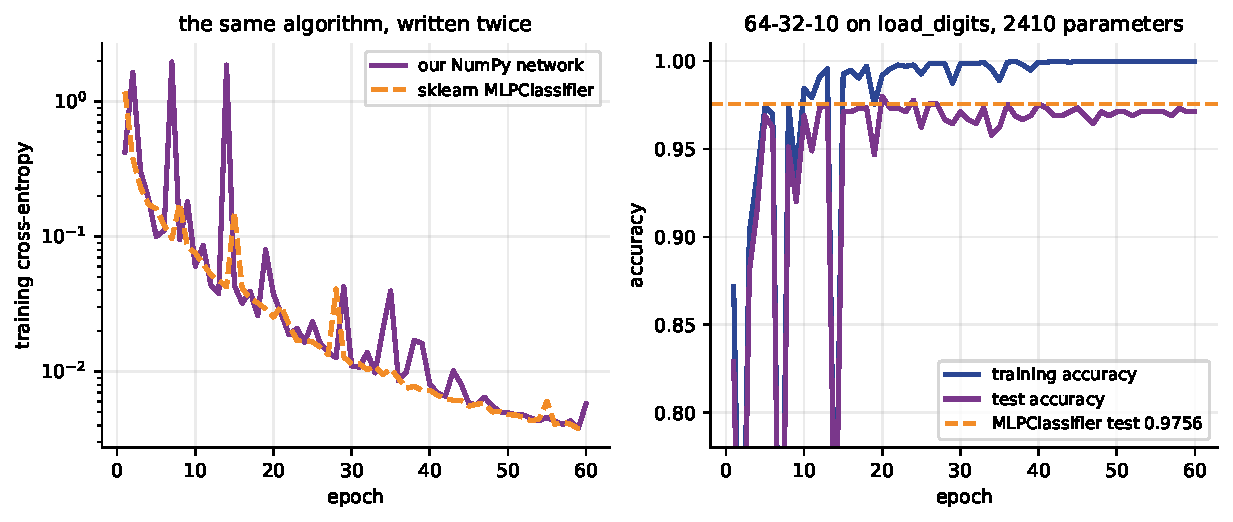
\includegraphics[width=0.92\textwidth]{losscurve.pdf}
  \caption{The training loss of the fourteen-line NumPy network against
    \texttt{MLPClassifier} on the same data with the same hyperparameters. Two
    independent implementations of the same algorithm, tracking each other for
    sixty epochs. The spikes are mini-batch noise at $\eta = 0.5$, present in
    both.}
  \label{fig:losscurve}
\end{figure}

\subsection{The same model from the library}

\begin{lstlisting}
from sklearn.neural_network import MLPClassifier
mlp = MLPClassifier(hidden_layer_sizes=(32,), activation="relu",
                    solver="sgd", learning_rate_init=0.5, batch_size=32,
                    max_iter=60, random_state=0)
mlp.fit(Xtr, ytr)
print(mlp.score(Xte, yte))
\end{lstlisting}
\begin{codeout}
MLPClassifier(hidden_layer_sizes=(32,), solver='sgd', lr=0.5, 60 epochs)
   test accuracy from scratch, NumPy : 0.9711
   test accuracy MLPClassifier       : 0.9756
   difference                        : +0.0044
   MLPClassifier final training loss : 0.0037
   our      final training loss      : 0.0058
   coefs_[0] shape (64, 32)  coefs_[1] shape (32, 10)
   MLPClassifier with its default Adam solver: 0.9733
   logistic regression, no hidden layer      : 0.9689
\end{codeout}

A difference of $+0.0044$ on $450$ test rows is \textbf{two rows}. The two
implementations differ only in how they shuffle the mini-batches and how they
initialise. Note also \texttt{coefs\_[0]} has shape $(64, 32)$ --- exactly the
$W^{(1)}$ of our code --- so you can pull the library's weights into our
forward pass and vice versa.

The last line is the honest control: \textbf{logistic regression with no
hidden layer at all scores $0.9689$.} The hidden layer bought $0.0022$ here,
which is one test row. Digits at $8\times8$ is very nearly linearly separable,
and a lecture that showed only the $0.9711$ would be quietly misleading. The
hidden layer earns its keep on \texttt{moons} (Section~\ref{sec:collapse}:
$0.8750 \to 0.9625$), not here.

\subsection{Gradient-check the whole network, not just the toy}

The nine-parameter check in Section~\ref{sec:gradcheck} was a proof of
concept. Do the same thing to the real network, on a batch of eight rows, over
sixty randomly chosen weight entries.

\begin{codeout}
64-32-10 network, batch of 8 rows, 60 randomly chosen weight entries
layer  entry        backprop            finite difference     |diff|
  W1   (25,27)   -0.001717812303     -0.001717812292     1.02e-11
  W1   ( 5,27)   -0.046692799725     -0.046692799716     9.74e-12
  W1   ( 1,17)   -0.000164852261     -0.000164852265     3.69e-12
  W1   ( 5, 9)   -0.035753919656     -0.035753919647     9.27e-12
  W1   (29,31)   +0.036876849891     +0.036876849885     5.85e-12
  ... 60 entries checked in total
largest absolute disagreement            : 2.796e-11
largest relative error where |grad|>1e-6 : 2.240e-08
many sampled entries are exactly 0.000000 in both columns: a dead ReLU,
or a border pixel that is 0 in all eight rows, has no gradient at all.
\end{codeout}

$2.796\times10^{-11}$ across sixty entries of a real network. The last two
lines are worth reading carefully rather than skipping: many sampled entries
came back as exactly $+0.000000000000$ in \emph{both} columns. Those are
border pixels that are $0$ in all eight rows of the batch, or ReLU units that
were negative for every row --- \textbf{dead} units. In both cases there
genuinely is no gradient, and the check correctly reports none. A zero in the
gradient is not automatically a bug.

\subsection{And the same model in the course's own library}

\begin{lstlisting}
from gradkit import nn, optim
model = nn.Sequential(nn.Dense(64, 32), nn.ReLU(), nn.Dense(32, 10))
gk.fit(model, (Xtr, ytr), "cross_entropy",
       optim.SGD(model.parameters(), lr=0.5), epochs=60, batch_size=32)
\end{lstlisting}
\begin{codeout}
gradkit nn.Sequential(Dense(64,32), ReLU(), Dense(32,10)), SGD lr=0.5
   test accuracy, gradkit           : 0.9667
   test accuracy, our NumPy version : 0.9711
   test accuracy, MLPClassifier     : 0.9756
three implementations of the same algorithm, three accuracies within
   0.0089 of each other.
   gradcheck(sigmoid) -> True
   gradcheck(tanh   ) -> True
   gradcheck(relu   ) -> True
   gradcheck compares each analytic derivative with a central
   finite difference -- the same check we did by hand in R11.
\end{codeout}

A spread of $0.0089$ on $450$ test rows is \textbf{four rows}. Nothing
separates the three implementations; they are the same algorithm with
different shuffling and different initialisation draws.

Note the last four lines. \texttt{gradkit} ships a \texttt{gradcheck} utility
that does to every one of its own primitives exactly what we did by hand in
Section~\ref{sec:gradcheck}: compares the analytic derivative against a
central finite difference. That is not a coincidence of design. It is the
standard way every autodiff library in existence is tested, including PyTorch
and JAX.

\begin{keyidea}
Use a library to \emph{read}, not to depend on. Three independent
implementations agreeing to four test rows is evidence that you understand the
algorithm; a single library producing a number you cannot reproduce is not.
\end{keyidea}

\begin{figure}[htbp]
  \centering
  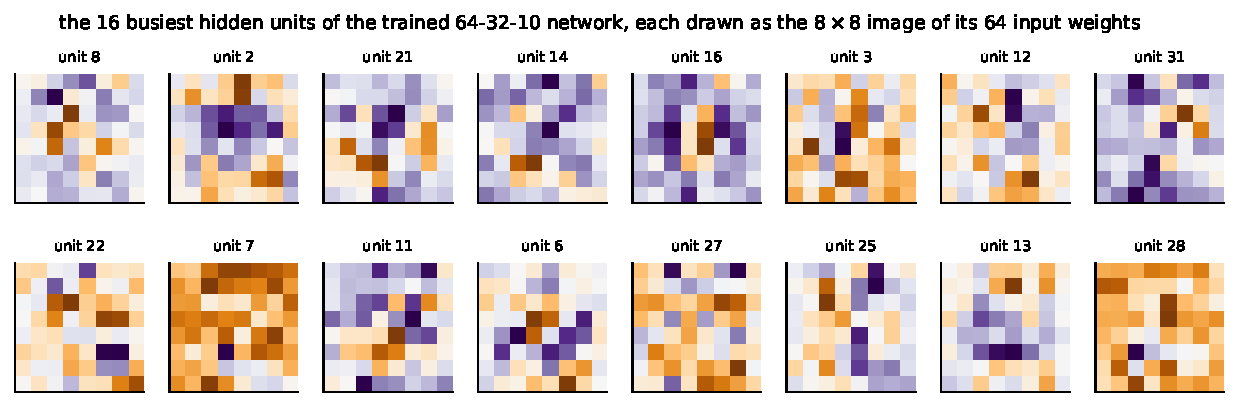
\includegraphics[width=0.98\textwidth]{hidden.pdf}
  \caption{Each tile is one hidden unit's $64$ input weights, folded back into
    the $8\times8$ image shape. They are stroke and blob detectors --- the
    features nobody specified, discovered because the gradient said so.}
  \label{fig:hidden}
\end{figure}

\subsection{Scaling matters more here than almost anywhere}
\label{sec:scaling}

The caution in Section~\ref{sec:tinynet} said an input twice as large gets a
gradient twice as large. Here is what that costs on real data.

\begin{codeout}
   logistic regression  test accuracy 0.9580
   MLP (16,)  scaled    test accuracy 0.9580
   MLP (64,32) scaled   test accuracy 0.9510
   MLP (64,32) RAW      test accuracy 0.9371
   scaling matters more to a neural network than to almost anything
   else, because the first layer's gradient is x times a delta.
\end{codeout}

Same architecture, same optimiser, same number of epochs: $0.9510$ scaled
against $0.9371$ raw. The reason is structural and you can point at it in the
derivation --- $\partial L/\partial w_{ij} = \delta_j x_i$ has $x_i$ as a
literal factor. A tree does not care about feature scale at all (it asks about
order); a network cares more than almost any other model in this course.

% =========================================================================
\section{Where the weights start}
\label{sec:init}

\subsection{Start everything at zero and nothing happens}

Take the $64$--$32$--$10$ network, the same data, thirty epochs. Change one
thing: initialise \textbf{every weight to $0$} instead of drawing them at
random. What test accuracy comes out?

\begin{codeout}
30 epochs, identical architecture, identical data, three initialisations
  init            train loss  train acc  test acc
  all zeros         2.3081      0.1010     0.1000
  all 0.1           2.4387      0.2517     0.2356
  He normal         0.0110      0.9985     0.9711
after training, are the 32 hidden units distinguishable?
  zeros init : max spread across hidden columns of W1 = 0.000e+00
  0.1   init : max spread across hidden columns of W1 = 0.000e+00
  He    init : max spread across hidden columns of W1 = 2.774e+00
  zeros init : columns 0 and 17 of W1 identical? True
  0.1   init : columns 0 and 17 of W1 identical? True
  He    init : columns 0 and 17 of W1 identical? False
chance accuracy on 10 balanced classes is 0.1000;
  the all-zeros network reached 0.1000, which is what predicting the
  commonest class gets: 0.1022
\end{codeout}

$\mathbf{0.1000}$. Chance. And it is not slow learning that more epochs would
fix --- it is \textbf{structurally} stuck.

\subsection{Symmetry, and why it never breaks}

\begin{worked}[The induction]
Suppose two hidden units $j$ and $k$ start with identical incoming weight
vectors, $w_{\cdot j} = w_{\cdot k}$, and identical biases.

\textbf{Forward.} For any input $x$, $z_j = w_{\cdot j}^\top x + b_j =
w_{\cdot k}^\top x + b_k = z_k$, so $a_j = a_k$. The two units compute the
same number on every row of the dataset.

\textbf{Backward.} Their outgoing weights are identical too (same argument
applied to the layer above), so by equation~\eqref{eq:bp1},
$\delta_j = \delta_k$.

\textbf{Update.} By equation~\eqref{eq:bp2}, $\nabla w_{ij} = a_i\delta_j =
a_i\delta_k = \nabla w_{ik}$ for every $i$. So both columns receive the
\emph{same} update and are \emph{still} identical afterwards.

By induction on the number of steps, they are identical forever.
\ensuremath{\square}
\end{worked}

The output confirms it empirically: after thirty epochs of training,
\texttt{columns 0 and 17 of W1 identical? True}, and the maximum spread across
all $32$ hidden columns is $\mathbf{0.000e+00}$.

\begin{keyidea}
It is not zero that is the problem, it is \textbf{equality}. All-$0.1$ fails
in exactly the same way (and reaches $0.2356$, a little above chance only
because the biases and the second layer can still do something). A $32$-unit
layer with identical columns is a $1$-unit layer wearing a costume.
\end{keyidea}

\subsection{The rule to use}

Break the symmetry by drawing the weights at random. But not from any
distribution: the variance matters, because the forward activations and the
backward gradients both get multiplied by these weights once per layer, and if
the scale is wrong they grow or shrink geometrically --- the same compounding
as Section~\ref{sec:vanish}.

\begin{itemize}[leftmargin=*]
  \item \textbf{He initialisation}, for ReLU:
    $w \sim \mathcal{N}(0,\; 2/n_{\text{in}})$. The factor $2$ compensates for
    ReLU zeroing out roughly half its inputs.
  \item \textbf{Xavier} (also called \textbf{Glorot}), for sigmoid and tanh:
    $w \sim \mathcal{N}(0,\; 1/n_{\text{in}})$, or the
    $2/(n_{\text{in}}+n_{\text{out}})$ variant that balances the forward and
    backward passes.
\end{itemize}

\begin{caution}
Biases \emph{may} start at zero, and usually should. They are not what breaks
the symmetry --- the weights are. Two units with identical weights and
different biases still compute perfectly correlated outputs and still receive
proportional gradients; the argument above barely changes. Randomise the
weights.
\end{caution}

\begin{figure}[htbp]
  \centering
  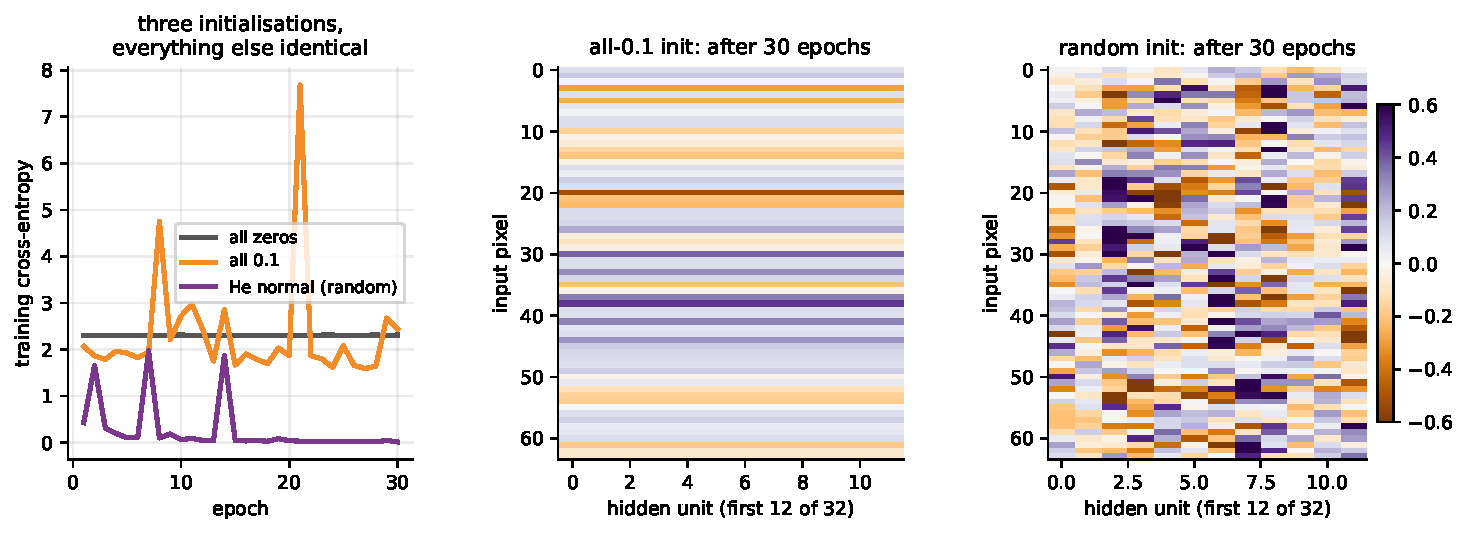
\includegraphics[width=0.98\textwidth]{init.pdf}
  \caption{The same architecture and data under three initialisations. The
    zero-initialised and constant-initialised networks never separate their
    hidden units; the He-initialised one does, and trains.}
  \label{fig:init}
\end{figure}

% =========================================================================
\section{Recurrent and feedback architecture}
\label{sec:rnn}

\subsection{Add one edge that points backwards}

Every network so far has been feedforward: the graph has no cycles. Add one
edge from a layer back to itself, delayed by one time step, and you have a
\textbf{recurrent} network:
\begin{equation}
  h_t = \varphi\!\left(W_{hh}h_{t-1} + W_{xh}x_t + b\right),
  \qquad
  y_t = W_{hy}h_t.
  \label{eq:rnn}
\end{equation}

\textbf{What changed.} The layer's input now includes its own previous output.
The network has a \textbf{state}, so its answer depends on the whole history,
not only the current input. That is what makes it suitable for
\textbf{sequences}: text, speech, sensor streams, log files.

\textbf{What did not change.} $W_{hh}$, $W_{xh}$, $W_{hy}$ and $b$ are the
\textbf{same at every time step}. A hundred-step sequence does not have a
hundred times as many parameters; it reuses one small set a hundred times,
exactly as a \texttt{for} loop reuses one body. This is called \textbf{weight
sharing} and it is why an RNN can process sequences of any length.

The syllabus calls this a \textbf{feedback} architecture, against the
\textbf{feedforward} networks of the rest of the lecture. Both names mean the
same thing.

\subsection{Unrolling, and backpropagation through time}

\begin{figure}[htbp]
  \centering
  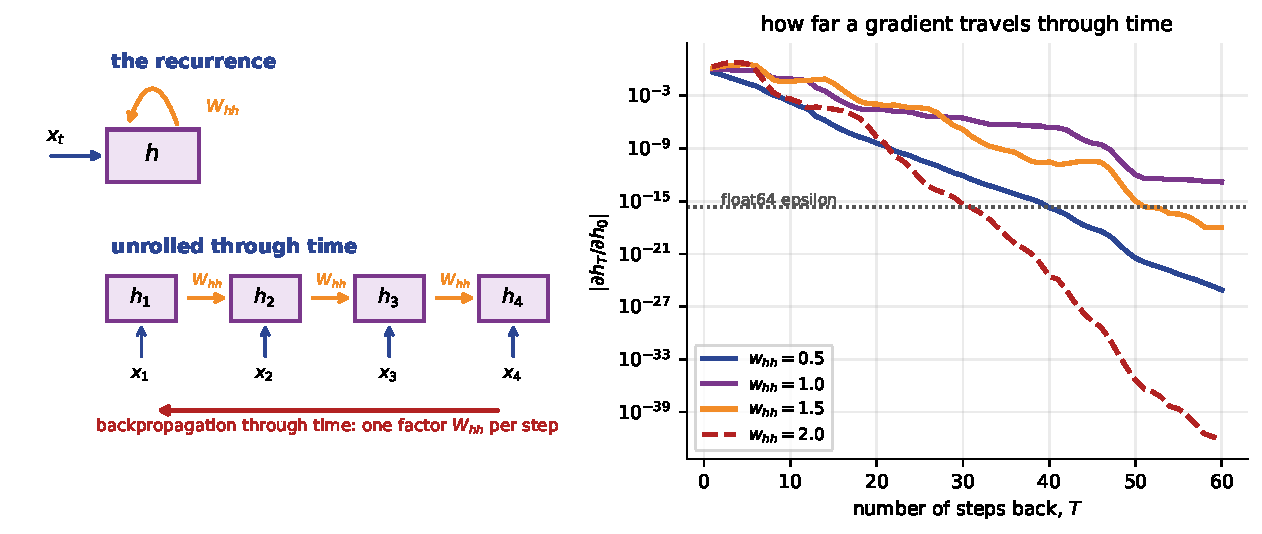
\includegraphics[width=0.86\textwidth]{rnn.pdf}
  \caption{The recurrent cell of equation~\eqref{eq:rnn}, and the same
    computation unrolled over $T$ steps into a feedforward network whose
    layers share their weights.}
  \label{fig:rnn}
\end{figure}

\begin{keyidea}
\textbf{Unroll} the loop over $T$ steps and you have an ordinary feedforward
network, $T$ layers deep, whose layers happen to share their weights.
Backpropagation then applies \emph{unchanged}: run it on the unrolled graph,
and \emph{sum} each shared weight's gradient over all the steps in which it
appeared. That is all \textbf{BPTT} --- backpropagation through time --- is.
There is no new algorithm here.
\end{keyidea}

The summation is the multivariable chain rule doing its job: a variable that
branches out to several places in the graph accumulates the gradients flowing
back from all of them.

\subsection{By hand: three steps, and the gradient back to the start}

Scalar case, so it fits on a line. One unit, $\tanh$ activation,
$w_{hh} = 0.9$, $w_{xh} = 1$, $b = 0$, $h_0 = 0$, and the input sequence
$x = (1, 0, 0)$ --- one signal at the first step and silence afterwards.

\begin{codeout}
h_t = tanh(w_hh h_{t-1} + w_xh x_t + b),   y_t = w_hy h_t
unrolled for T = 3 with x = (1, 0, 0), w_hh = 0.9, w_xh = 1, b = 0:
   h1 = tanh(0.9 * 0.000000 + 1.0 * 1.0) = 0.761594
   h2 = tanh(0.9 * 0.761594 + 1.0 * 0.0) = 0.595041
   h3 = tanh(0.9 * 0.595041 + 1.0 * 0.0) = 0.489602
dh3/dh0 = prod_t w_hh (1 - h_t^2) = 0.150353
\end{codeout}

\begin{worked}[Where $0.150353$ comes from]
Differentiate equation~\eqref{eq:rnn} in the scalar case:
$\partial h_t/\partial h_{t-1} = w_{hh}\,\tanh'(\cdot) = w_{hh}(1 - h_t^2)$.
Chaining over three steps,
\[
  \frac{\partial h_T}{\partial h_0} = \prod_{t=1}^{T} w_{hh}(1 - h_t^2).
\]
Compute the three factors. $1 - h_1^2 = 1 - 0.761594^2 = 0.420002$;
$1 - h_2^2 = 1 - 0.595041^2 = 0.645926$; $1 - h_3^2 = 1 - 0.489602^2 =
0.760290$. So
\[
  (0.9)(0.4200)\times(0.9)(0.6459)\times(0.9)(0.7603)
  = 0.729 \times 0.206246 = \mathbf{0.150353}.
\]
\end{worked}

Read the two halves of that against each other. The input at $t = 1$ still
plainly echoes in the state: $h_3 = 0.4896$ is a long way from zero, and it
got there entirely from $x_1$. \textbf{The information survives.} But the
gradient that would teach the network to \emph{use} that information has
already shrunk to $15\%$ after only three steps.

\subsection{There are exactly two things that product can do}

\begin{codeout}
how far back does a gradient survive?  |dh_T/dh_0| for a scalar tanh RNN
    T     w_hh=0.5      w_hh=1.0      w_hh=1.5      w_hh=2.0
     1   4.9803e-01   9.9606e-01   1.4941e+00   1.9921e+00
     5   2.6534e-02   7.9059e-01   3.7933e+00   4.4321e+00
    10   2.0326e-04   8.5842e-02   4.2845e-02   4.4101e-04
    20   3.9998e-09   2.5262e-05   1.1633e-04   2.0875e-08
    50   3.3054e-22   1.0712e-12   1.0959e-15   4.1206e-36
   100   8.5708e-43   3.9559e-20   9.4559e-34   1.5963e-74
the product of T numbers each below 1 decays geometrically;
the product of T numbers each above 1 grows geometrically. There is no
third case: |w (1-h^2)| = 1 exactly is a measure-zero accident.
\end{codeout}

A product of $T$ numbers each below $1$ decays geometrically: the
\textbf{vanishing gradient}. A product of $T$ numbers each above $1$ grows
geometrically: the \textbf{exploding gradient}. Watch $w_{hh} = 2.0$ do both
--- it more than doubles between $T = 1$ and $T = 5$, from $1.99$ to $4.43$,
and then $\tanh$ saturates, $1 - h^2$ collapses towards zero, and the product
crashes to $4.1\times10^{-36}$ by $T = 50$.

There is no third case. $|w_{hh}(1-h^2)| = 1$ exactly, sustained over many
steps, is a measure-zero accident.

\begin{caution}
The two failures are not symmetric in difficulty. \textbf{Exploding is easy to
fix}: clip the gradient norm to a fixed maximum before the update and carry
on. \textbf{Vanishing is not fixable that way} --- you cannot amplify
information that is no longer there. That asymmetry is why gated
architectures, LSTM and GRU, were invented: they give the state an additive
path through time on which the derivative is close to $1$ by construction.
\end{caution}

\subsection{Measured: how far back an RNN can actually remember}

A task designed so that only the memory is being tested. Read a binary
sequence of length $T$ and report its \textbf{first} symbol. Every other
symbol is noise. The task does not get harder as $T$ grows --- the answer is
sitting at $t = 1$ every single time. The only thing that changes is how far
the gradient has to travel back.

\begin{codeout}
task: read a binary sequence of length T, report its FIRST symbol.
one tanh recurrent unit bank of width 8, plain BPTT, 400 epochs.
      T   held-out accuracy   ||gradient at t=1|| at epoch 0
      2       1.0000              3.335e-03
      5       1.0000              3.976e-04
     10       1.0000              2.088e-05
     20       0.5500              9.086e-08
     40       0.4925              1.527e-12
the information needed is present at t = 1 in every case.
what changes with T is only how far the gradient has to travel back.
\end{codeout}

Perfect to $T = 10$. At $T = 20$ the gradient arriving at the first step is
$9\times10^{-8}$ and the accuracy has fallen to $0.5500$. At $T = 40$ the
gradient is $1.5\times10^{-12}$ and the network scores $\mathbf{0.4925}$: a
coin.

\textbf{This is the vanishing gradient measured on a task, not drawn on a
diagram.} It is also the honest boundary of what a plain RNN can do, and the
reason the sequence models you will meet later --- LSTM, GRU, and attention
--- exist at all. For this syllabus, the recurrent architecture is one row:
know equation~\eqref{eq:rnn}, know that unrolling reduces BPTT to ordinary
backpropagation with summed gradients, and know why the product of $T$ factors
has only two behaviours.

% =========================================================================
\section{Summary}
\label{sec:summary}

\begin{enumerate}[leftmargin=*]
  \item A unit is $\varphi(w^\top x + b)$. With $\varphi = $ identity it is
    linear regression, with $\sigma$ it is logistic regression, with a step it
    is a \textbf{perceptron}.
  \item The perceptron rule $w \leftarrow w + \eta(y-\hat y)x$ is
    mistake-driven and is \emph{not} a gradient. On AND it converges in
    $\mathbf{6}$ epochs and $\mathbf{11}$ updates to $2x_1 + x_2 - 3 \ge 0$;
    on separable iris, $6$ epochs to accuracy $1.0000$, matching
    \texttt{sklearn}'s \texttt{Perceptron}.
  \item If the data is not linearly separable the rule \textbf{cycles
    forever}. On XOR it ends at $0.50$, revisiting only two states in a
    thousand epochs; the best of all $531\,441$ lines searched gets only
    $\mathbf{0.75}$. Two separate failures.
  \item Two hidden units fix XOR by mapping $(0,1)$ and $(1,0)$ to the same
    point $(1,0)$. A hidden layer \textbf{re-represents}; the output layer is
    still just linear. With one hidden unit the loss stalls at $0.1186$,
    barely below its starting $0.1257$; with two it reaches
    $4.42\times10^{-4}$.
  \item Without a non-linearity, depth is free of charge and worth nothing:
    three layers with $77$ parameters equal one with $10$ to
    $\mathbf{7.1\times10^{-15}}$, and $W_{\text{eff}}$ has rank $2$. On moons,
    $1058$ identity-activated parameters beat $3$ by $0.0025$; ReLU beats them
    by $0.0875$.
  \item $\sigma' \le \mathbf{0.25}$, $\tanh' \le 1$,
    $\mathrm{ReLU}' \in \{0,1\}$. Ten sigmoid layers attenuate the first-layer
    gradient to $\mathbf{6.96\times10^{-7}}$ against ReLU's
    $1.90\times10^{-2}$: a ratio of $\mathbf{27\,320}$, and
    $0.25^{10} = 9.54\times10^{-7}$ predicted it in advance.
  \item Consequence, measured on real data: three sigmoid hidden layers on
    digits score $\mathbf{0.1000}$ --- chance, at loss $\ln 10$ --- while
    three ReLU layers score $0.9733$.
  \item Backpropagation is the chain rule read \textbf{left to right}: one
    forward and one backward pass give every parameter's derivative, at about
    twice the cost of the forward pass alone.
  \item On the $2$--$2$--$1$ network: $a_1 = 0.5$, $a_2 = 0.7310585786$,
    $a_3 = 0.4653966177$, $L = \mathbf{0.1429003882}$,
    $\delta_3 = -0.1330107147$, $\delta_1 = -0.0133010715$,
    $\delta_2 = +0.0156908963$, and nine gradients from $-0.1330$ to
    $+0.0314$.
  \item Two rules, any depth:
    $\delta^{(\ell)} = (W^{(\ell+1)}\delta^{(\ell+1)})\odot\varphi'(z^{(\ell)})$
    and $\nabla W^{(\ell)} = a^{(\ell-1)}\delta^{(\ell)\top}$, with
    $\nabla b^{(\ell)} = \delta^{(\ell)}$ summed over the batch. For softmax
    with cross-entropy, $\partial L/\partial z = p - y$.
  \item All nine hand gradients matched central differences to
    $\mathbf{4.107\times10^{-11}}$ and \texttt{gradkit} autodiff to
    $\mathbf{0.000e{+}00}$, bit for bit. The $64$--$32$--$10$ network's
    gradients matched to $2.796\times10^{-11}$ over sixty entries.
    \textbf{Always gradient-check.}
  \item Fourteen lines of NumPy reach $\mathbf{0.9711}$ on
    \texttt{load\_digits} with $2410$ parameters; \texttt{MLPClassifier} gets
    $0.9756$ and \texttt{gradkit} $0.9667$ --- a spread of four test rows.
    Honest control: logistic regression with no hidden layer gets $0.9689$.
  \item Training accuracy hits $1.0000$ at epoch 60 while test accuracy falls
    from its peak of $0.9800$ at epoch 20 to $0.9711$. That is overfitting and
    the case for early stopping.
  \item All-zero initialisation gives $\mathbf{0.1000}$ and all-$0.1$ gives
    $0.2356$, because identical units receive identical gradients and stay
    identical forever --- confirmed by a column spread of $0.000e{+}00$ after
    training. Use He for ReLU, Xavier for sigmoid and tanh; biases may start
    at zero.
  \item Scale your features. $\partial L/\partial w_{ij} = \delta_j x_i$ has
    the input as a literal factor: raw digits score $0.9371$ against scaled
    $0.9510$.
  \item An RNN shares one weight set across time; BPTT is backpropagation on
    the unrolled graph with each shared gradient summed.
    $\partial h_T/\partial h_0$ is a product of $T$ factors, so it vanishes or
    explodes and there is no third case. Measured on a remember-the-first-bit
    task: accuracy $1.0000$ at $T=10$ and $\mathbf{0.4925}$ at $T=40$.
\end{enumerate}

% =========================================================================
\section{Practice questions}
\label{sec:practice}

Work these with a pen before running anything. Solutions with full working
follow in Section~\ref{sec:solutions}. Questions 3, 4 and 5 are
forward-and-backward passes by hand; those three are the examinable core of
this lecture and you should be able to do all of them without notes.

\begin{enumerate}[leftmargin=*]
  \item \textbf{The perceptron rule on OR.} Four rows: $(0,0)\to 0$,
    $(0,1)\to 1$, $(1,0)\to 1$, $(1,1)\to 1$. Start from $w = (0,0)$, $b = 0$,
    $\eta = 1$, and sweep the rows in the order given. Trace every row of
    every epoch until a full sweep makes no update. State the number of epochs
    and the number of weight updates, and write down the final decision rule.
    Compare the count with AND's $6$ epochs and $11$ updates and explain the
    difference in one sentence.

  \item \textbf{XOR is not the only unlearnable function.} (a) Reproduce the
    four-inequality proof that no single unit computes XOR. (b) There are
    sixteen Boolean functions of two variables. How many of them can a single
    perceptron compute, and which ones cannot? Justify your count.

  \item \textbf{Backpropagation by hand, with the target moved.} Take the
    network of Section~\ref{sec:tinynet} with exactly the same nine parameters
    and the same inputs $x = (1.0, 2.0)$, but change the target from
    $t = 1.0$ to $t = \mathbf{0.0}$. Compute the forward pass, the loss, and
    all nine gradients. Give every number to ten decimal places, and say
    which quantities from the worked example you were able to reuse unchanged
    and why.

  \item \textbf{Backpropagation by hand, with a tanh hidden layer.} A
    $2$--$1$--$1$ network: $z_1 = w_1x_1 + w_2x_2 + b_1$, $a_1 = \tanh(z_1)$,
    $z_2 = v_1a_1 + b_2$, $a_2 = \sigma(z_2)$, $L = \tfrac12(a_2-t)^2$. Take
    $x = (1, -1)$, $t = 1$, $w_1 = 0.5$, $w_2 = 0.5$, $b_1 = 0$, $v_1 = 2.0$,
    $b_2 = 0$. Compute the forward pass and all five gradients. You should be
    able to do the whole of this one in your head up to the sigmoid.

  \item \textbf{Backpropagation by hand, with ReLU and two outputs.} A
    $1$--$2$--$1$ network with ReLU hidden units:
    $z_j = w_jx + b_j$, $a_j = \max(0, z_j)$ for $j = 1, 2$;
    $z_3 = v_1a_1 + v_2a_2 + b_3$, $\hat y = z_3$ (identity output);
    $L = \tfrac12(\hat y - t)^2$. Take $x = 2$, $t = 1$, $w_1 = 1$,
    $b_1 = -1$, $w_2 = -1$, $b_2 = -1$, $v_1 = 3$, $v_2 = 3$, $b_3 = 0$.
    Compute the forward pass and all seven gradients. Explain what happened to
    unit 2 and what that means for its parameters.

  \item \textbf{Predicting the attenuation.} A network has $L$ hidden layers,
    all sigmoid. (a) Give an upper bound on the factor by which the gradient
    can be attenuated between the top hidden layer and the first, in terms of
    $L$, ignoring the weights. (b) Evaluate it for $L = 10$ and compare with
    the measured $8.3167\times10^{-7}$ of Section~\ref{sec:vanish}. (c) The
    measured value is \emph{smaller} than $0.25^{10}$ would suggest is
    possible from the activations alone at some layers and larger at others.
    Name the other factor in equation~\eqref{eq:bp1} that accounts for the
    difference.

  \item \textbf{Counting and collapsing.} (a) How many parameters does a
    $20$--$50$--$50$--$3$ fully connected network have? Show the arithmetic.
    (b) If every activation is the identity, what is the maximum rank of the
    effective weight matrix, and how many parameters does the equivalent
    single layer have? (c) State in one sentence what the $20$--$50$--$50$--$3$
    identity network can compute that the single layer cannot.

  \item \textbf{Softmax and cross-entropy by hand.} A three-class classifier
    outputs logits $z = (1.0,\, 2.0,\, 3.0)$ for a row whose true class is the
    \emph{first}. (a) Compute the softmax probabilities to six decimal places.
    (b) Compute the cross-entropy loss. (c) Write down $\partial L/\partial z$
    without differentiating anything, and state the property of the three
    components that must hold for any softmax--cross-entropy gradient.

  \item \textbf{Diagnosing a dead network.} A student reports that their
    $784$--$128$--$10$ network trains to exactly $0.1135$ test accuracy on a
    ten-class problem, no matter how many epochs they run, and that the loss
    sits at $2.303$ from the first epoch. Give the two most likely causes, say
    what single diagnostic you would run to distinguish them, and state what
    each cause would produce.

  \item \textbf{The recurrent product.} A scalar tanh RNN has
    $w_{hh} = 1.2$ and a state that happens to stay at $h_t = 0.5$ for every
    $t$. (a) Compute the per-step factor $w_{hh}(1 - h_t^2)$. (b) Compute
    $|\partial h_T/\partial h_0|$ for $T = 10$ and $T = 50$. (c) State which
    of the two failure modes this is, and what the standard fix is. (d) Repeat
    (a) and (b) for $h_t = 0.7$ and say what changed.
\end{enumerate}

% =========================================================================
\section{Solutions}
\label{sec:solutions}

\paragraph{1. The perceptron rule on OR.}
Trace it. Write the state as $(w_1, w_2 \mid b)$, starting at
$(0,0 \mid 0)$.

\emph{Epoch 1.} Row $(0,0)$, target $0$: $z = 0 \ge 0$ so $\hat y = 1$,
error $-1$, and since $x = (0,0)$ only the bias moves:
$(0,0 \mid -1)$. Row $(0,1)$, target $1$: $z = 0 - 1 = -1$, $\hat y = 0$,
error $+1$: $w \leftarrow (0,0)+(0,1) = (0,1)$, $b \leftarrow 0$, giving
$(0,1 \mid 0)$. Row $(1,0)$, target $1$: $z = 0 + 0 = 0 \ge 0$, $\hat y = 1$,
correct, no change. Row $(1,1)$, target $1$: $z = 0 + 1 + 0 = 1 \ge 0$,
correct. Two updates.

\emph{Epoch 2.} Row $(0,0)$: $z = 0 \ge 0$, $\hat y = 1$, error $-1$:
$(0,1 \mid -1)$. Row $(0,1)$: $z = 1 - 1 = 0 \ge 0$, $\hat y = 1$, correct.
Row $(1,0)$: $z = 0 - 1 = -1$, $\hat y = 0$, error $+1$:
$w \leftarrow (1,1)$, $b \leftarrow 0$, giving $(1,1 \mid 0)$. Row $(1,1)$:
$z = 2 \ge 0$, correct. Two updates.

\emph{Epoch 3.} Row $(0,0)$: $z = 0 \ge 0$, error $-1$: $(1,1 \mid -1)$.
Row $(0,1)$: $z = 1 - 1 = 0 \ge 0$, correct. Row $(1,0)$: $z = 0$, correct.
Row $(1,1)$: $z = 1 \ge 0$, correct. One update.

\emph{Epoch 4.} Row $(0,0)$: $z = -1 < 0$, $\hat y = 0$, correct. All four
rows: $-1, 0, 0, 1$, giving $0, 1, 1, 1$. Correct. \textbf{No updates.}

So OR takes \textbf{4 epochs and 5 weight updates}, converging to
$x_1 + x_2 - 1 \ge 0$.

Why fewer than AND? AND has a single positive row at the far corner and three
negatives, so the bias has to be pushed down a long way ($b = -3$ at
convergence) while the weights are simultaneously pushed up, and the two
requirements fight each other for five epochs. OR has three positives and one
negative and needs only $b = -1$. Both problems are separable, so the
convergence theorem guarantees termination in both cases; the bound
$(R/\gamma)^2$ is simply smaller for OR because its margin is larger.

\paragraph{2. XOR and the sixteen Boolean functions.}

(a) Suppose $w_1x_1 + w_2x_2 + b \ge 0$ exactly on the positive rows. Then
$b < 0$ from $(0,0)$; $w_2 + b \ge 0$ from $(0,1)$; $w_1 + b \ge 0$ from
$(1,0)$; $w_1 + w_2 + b < 0$ from $(1,1)$. Adding the middle two gives
$w_1 + w_2 \ge -2b$, and substituting into the fourth gives $-2b + b < 0$,
so $b > 0$, contradicting the first. \ensuremath{\square}

(b) A perceptron on two binary inputs computes exactly the
\textbf{linearly separable} Boolean functions of two variables. Of the
sixteen, \textbf{fourteen} are separable and \textbf{two} are not: XOR and
its complement XNOR.

The count is easiest to see by elimination. The two constant functions, the
four functions depending on one input only ($x_1$, $\lnot x_1$, $x_2$,
$\lnot x_2$), and the eight functions that isolate exactly one corner or
exactly three corners (AND, NAND, OR, NOR, and the four implications) are all
half-planes: any single corner can be cut off by a line, and so can any three.
That is $2 + 4 + 8 = 14$. The only remaining functions pick out two
\emph{diagonally opposite} corners, and by the argument of part (a) no line
can do that. Those two are XOR and XNOR.

\paragraph{3. Backpropagation with $t = 0.0$.}

This is the exercise the lecture sets, and the point of it is that
\textbf{the entire forward pass is unchanged}: $t$ appears nowhere in
equations~\eqref{eq:tf1}--\eqref{eq:tf3}. So

\[
  z_1 = 0.0, \quad a_1 = 0.5000000000, \quad
  z_2 = 1.0, \quad a_2 = 0.7310585786,
\]
\[
  z_3 = -0.1386351472, \quad a_3 = 0.4653966177.
\]

Only the loss changes:
\[
  L = \tfrac12(0.4653966177 - 0.0)^2 = \tfrac12(0.2165940118)
    = \mathbf{0.1082970059}.
\]

Now the backward pass. Exactly one number changes, and everything else follows
from it:
\[
  \frac{\partial L}{\partial a_3} = a_3 - t = 0.4653966177 - 0.0
  = \mathbf{+0.4653966177}
\]
which is positive now, because the output is \emph{above} the target.

$\partial a_3/\partial z_3 = a_3(1-a_3) = +0.2488026059$ --- \textbf{reused
unchanged}, because it depends only on $a_3$.
\[
  \delta_3 = (0.4653966177)(0.2488026059) = \mathbf{+0.1157918913}.
\]

Output layer:
\begin{align*}
  \partial L/\partial v_1 &= \delta_3 a_1 = (0.1157918913)(0.5)
    = \mathbf{+0.0578959456}\\
  \partial L/\partial v_2 &= \delta_3 a_2 = (0.1157918913)(0.7310585786)
    = \mathbf{+0.0846506555}\\
  \partial L/\partial b_2 &= \delta_3 = \mathbf{+0.1157918913}
\end{align*}

Hidden deltas. The factors $v_j$ and $a_j(1-a_j)$ are \textbf{reused
unchanged} --- they are properties of the forward pass, not of the target:
\begin{align*}
  \delta_1 &= \delta_3 v_1 a_1(1-a_1) = (0.1157918913)(0.4)(0.25)
    = \mathbf{+0.0115791891}\\
  \delta_2 &= \delta_3 v_2 a_2(1-a_2)
    = (0.1157918913)(-0.6)(0.1966119332) = \mathbf{-0.0136596406}
\end{align*}

Input layer:
\begin{align*}
  \partial L/\partial w_{11} &= \delta_1 x_1 = \mathbf{+0.0115791891}
  & \partial L/\partial w_{12} &= \delta_2 x_1 = \mathbf{-0.0136596406}\\
  \partial L/\partial w_{21} &= \delta_1 x_2 = \mathbf{+0.0231583783}
  & \partial L/\partial w_{22} &= \delta_2 x_2 = \mathbf{-0.0273192811}\\
  \partial L/\partial b_{11} &= \delta_1 = \mathbf{+0.0115791891}
  & \partial L/\partial b_{12} &= \delta_2 = \mathbf{-0.0136596406}
\end{align*}

\textbf{What was reused, and why.} Everything except $\partial L/\partial a_3$
and the loss value. The forward pass, all three activations, both local
derivatives $a_j(1-a_j)$, and the whole routing structure are properties of
the \emph{network and the input}. The target enters at exactly one place, in
one subtraction, and its effect propagates as a scalar multiplier. That is
worth internalising: it is why a network can be trained on a new labelling of
the same inputs without recomputing anything structural, and it is why
$\delta$ at the top is called the ``error signal''.

Sanity checks you should apply: every gradient has flipped sign relative to
the worked example (the output must now go down instead of up); the magnitudes
are smaller because $|a_3 - t| = 0.4654$ is smaller than $0.5346$; and
$\partial L/\partial w_{21}$ is still exactly twice
$\partial L/\partial w_{11}$, because $x_2$ is still twice $x_1$.

\paragraph{4. Backpropagation with a tanh hidden layer.}

\emph{Forward.} $z_1 = (0.5)(1) + (0.5)(-1) + 0 = \mathbf{0}$, so
$a_1 = \tanh(0) = \mathbf{0}$ exactly. Then $z_2 = (2.0)(0) + 0 = \mathbf{0}$,
so $a_2 = \sigma(0) = \mathbf{0.5}$ exactly, and
\[
  L = \tfrac12(0.5 - 1)^2 = \tfrac12(0.25) = \mathbf{0.125}.
\]

\emph{Backward.} $\partial L/\partial a_2 = a_2 - t = 0.5 - 1 =
\mathbf{-0.5}$. $\partial a_2/\partial z_2 = a_2(1-a_2) = (0.5)(0.5) =
\mathbf{0.25}$. So
\[
  \delta_2 = (-0.5)(0.25) = \mathbf{-0.125}.
\]

Output layer:
\[
  \frac{\partial L}{\partial v_1} = \delta_2 a_1 = (-0.125)(0)
  = \mathbf{0}, \qquad
  \frac{\partial L}{\partial b_2} = \delta_2 = \mathbf{-0.125}.
\]

The gradient on $v_1$ is \emph{zero}. That is correct and instructive: the
hidden unit is outputting exactly $0$, so changing the weight that multiplies
it changes nothing, to first order. The rule ``gradient of a weight = delta
$\times$ the activation it multiplies'' predicted this before any arithmetic.

Hidden delta. $\tanh'(z_1) = 1 - \tanh^2(0) = 1 - 0 = \mathbf{1}$, the maximum
value tanh's derivative can take:
\[
  \delta_1 = \delta_2 \cdot v_1 \cdot \tanh'(z_1)
  = (-0.125)(2.0)(1) = \mathbf{-0.25}.
\]

Input layer:
\begin{align*}
  \frac{\partial L}{\partial w_1} &= \delta_1 x_1 = (-0.25)(1)
    = \mathbf{-0.25}\\
  \frac{\partial L}{\partial w_2} &= \delta_1 x_2 = (-0.25)(-1)
    = \mathbf{+0.25}\\
  \frac{\partial L}{\partial b_1} &= \delta_1 = \mathbf{-0.25}
\end{align*}

Five gradients: $(-0.25, +0.25, -0.25, 0, -0.125)$ for
$(w_1, w_2, b_1, v_1, b_2)$. Note the two input weights have opposite signs
purely because $x_2 = -x_1$, and note that the hidden layer passed
\emph{four times} more gradient down than the equivalent sigmoid unit would
have ($\tanh' = 1$ against $\sigma' \le 0.25$). That factor of four per layer
is exactly why tanh is preferred over sigmoid for hidden layers when you are
not using ReLU.

\paragraph{5. Backpropagation with ReLU.}

\emph{Forward.} $z_1 = (1)(2) + (-1) = \mathbf{1}$, so $a_1 = \max(0,1) =
\mathbf{1}$. $z_2 = (-1)(2) + (-1) = \mathbf{-3}$, so $a_2 = \max(0,-3) =
\mathbf{0}$. Then
\[
  z_3 = (3)(1) + (3)(0) + 0 = \mathbf{3}, \qquad \hat y = 3,
\]
\[
  L = \tfrac12(3 - 1)^2 = \tfrac12(4) = \mathbf{2}.
\]

\emph{Backward.} The output activation is the identity, so its derivative is
$1$ and
\[
  \delta_3 = \frac{\partial L}{\partial z_3} = \hat y - t = 3 - 1
  = \mathbf{+2}.
\]

Output layer:
\begin{align*}
  \frac{\partial L}{\partial v_1} &= \delta_3 a_1 = (2)(1) = \mathbf{+2}\\
  \frac{\partial L}{\partial v_2} &= \delta_3 a_2 = (2)(0) = \mathbf{0}\\
  \frac{\partial L}{\partial b_3} &= \delta_3 = \mathbf{+2}
\end{align*}

Hidden deltas. $\mathrm{ReLU}'(z_1) = \mathbf{1}[1 > 0] = 1$;
$\mathrm{ReLU}'(z_2) = \mathbf{1}[-3 > 0] = 0$:
\begin{align*}
  \delta_1 &= \delta_3 v_1 \cdot 1 = (2)(3)(1) = \mathbf{+6}\\
  \delta_2 &= \delta_3 v_2 \cdot 0 = \mathbf{0}
\end{align*}

Input layer:
\begin{align*}
  \frac{\partial L}{\partial w_1} &= \delta_1 x = (6)(2) = \mathbf{+12}
  & \frac{\partial L}{\partial b_1} &= \delta_1 = \mathbf{+6}\\
  \frac{\partial L}{\partial w_2} &= \delta_2 x = \mathbf{0}
  & \frac{\partial L}{\partial b_2} &= \delta_2 = \mathbf{0}
\end{align*}

Seven gradients: $(+12, +6, 0, 0, +2, 0, +2)$ for
$(w_1, b_1, w_2, b_2, v_1, v_2, b_3)$.

\textbf{What happened to unit 2.} Its pre-activation was $-3$, so ReLU
switched it off. It contributed nothing to the output, and consequently
\emph{all three} parameters attached to it --- $w_2$, $b_2$ and $v_2$ ---
received a gradient of exactly zero. They will not move on this step.

If that were true for \emph{every} row in the training set, unit 2 would be a
\textbf{dead ReLU}: permanently off, permanently zero-gradient, and
permanently unable to recover, because the only thing that could switch it
back on is an update to $w_2$ or $b_2$, and those updates are zero. This is
the standard failure mode of ReLU networks. It is why Leaky ReLU
($\max(\alpha z, z)$ with small $\alpha$) exists, and it is exactly what
produced the ``entries that are $0.000000$ in both columns'' in the
whole-network gradient check of Section~\ref{sec:mlp}. Note also that in a
mini-batch the gradient is summed over rows, so a unit only dies if it is off
for \emph{all} of them.

\paragraph{6. Predicting the attenuation.}

(a) Each backward step through a sigmoid layer multiplies the gradient by
$\sigma'(z) \le 1/4$ elementwise, and by the weight matrix. Ignoring the
weights, the attenuation between the top hidden layer and the first, across
$L - 1$ layer boundaries plus the top layer's own activation, is bounded by
$(1/4)^{L}$ at worst and $(1/4)^{L-1}$ counting boundaries only. The
examinable statement is: \textbf{the attenuation is at most $0.25$ per layer
and compounds geometrically}, so it is $O(4^{-L})$.

(b) For $L = 10$: $0.25^{10} = 9.5367\times10^{-7}$ and
$0.25^{9} = 3.8147\times10^{-6}$. The measured attenuation from layer 10 to
layer 1 was $8.3167\times10^{-7}$, which sits between the two and very close
to $0.25^{10}$. So the arithmetic predicts the measurement to within about
$15\%$.

(c) The other factor is the \textbf{weight matrix} $W^{(\ell+1)}$ in
equation~\eqref{eq:bp1}. Each backward step multiplies by $W^{\top}$ as well
as by $\varphi'$, and the weights can be larger or smaller than $1$ in norm.
In this experiment their contribution happened to be mildly amplifying
(otherwise the measured $8.32\times10^{-7}$ would have been below
$0.25^{10}$), which is why the sigmoid gradient at layer 10 was
$0.8370$ --- far larger than the ReLU network's $0.0289$ --- and yet the
first layer still received only $6.96\times10^{-7}$. The activations do the damage; the weights only
modulate it.

\paragraph{7. Counting and collapsing.}

(a) Three weight matrices and three bias vectors:
\[
  \underbrace{20{\cdot}50 + 50}_{1050}
  + \underbrace{50{\cdot}50 + 50}_{2550}
  + \underbrace{50{\cdot}3 + 3}_{153}
  = \mathbf{3753}.
\]

(b) $W_{\text{eff}} = W_1W_2W_3$ is $20 \times 3$, and its rank is at most
$\min(20, 50, 50, 3) = \mathbf{3}$. Here the bottleneck is the output width,
not a hidden layer, so nothing is lost that was not already lost. The
equivalent single layer is $20 \to 3$ and has $20{\cdot}3 + 3 = \mathbf{63}$
parameters. So $3753$ parameters are being spent to express a function that
$63$ express exactly --- a factor of about $60$ in wasted memory, wasted
arithmetic and wasted gradient computation.

(c) \textbf{Nothing.} That is the entire point of Section~\ref{sec:collapse}:
the two functions are identical, not merely similar. The deep identity network
can compute exactly the set of affine maps $\mathbb{R}^{20} \to \mathbb{R}^3$
of rank at most $3$, and so can the single layer. The only differences are
practical: the deep version has a different optimisation landscape and
different numerical conditioning, both of which are disadvantages here.

\paragraph{8. Softmax and cross-entropy by hand.}

(a) Subtract the maximum logit before exponentiating --- this is what every
library does, and it prevents overflow without changing the answer, because
$e^{z_c - m}/\sum_k e^{z_k - m} = e^{z_c}/\sum_k e^{z_k}$. With $m = 3$:
$e^{-2} = 0.135335$, $e^{-1} = 0.367879$, $e^{0} = 1$. Their sum is
$1.503215$. So
\[
  p = (0.090031,\; 0.244728,\; 0.665241).
\]
Check: they sum to $1.000000$.

(b) The true class is the first, so
\[
  L = -\log p_1 = -\log(0.090031) = \mathbf{2.407606}.
\]
Sanity check: a uniform guess over three classes would give
$-\log(1/3) = 1.098612$, so this prediction is substantially worse than
guessing --- as it should be, since the model put its highest probability on
the wrong class.

(c) By equation~\eqref{eq:softmaxgrad}, with $y = (1, 0, 0)$:
\[
  \frac{\partial L}{\partial z} = p - y
  = (0.090031 - 1,\; 0.244728,\; 0.665241)
  = (\mathbf{-0.909969},\; \mathbf{+0.244728},\; \mathbf{+0.665241}).
\]

The property that must always hold: \textbf{the components sum to zero}.
$-0.909969 + 0.244728 + 0.665241 = 0.000000$. This is forced, because $p$ sums
to $1$ and $y$ sums to $1$. It has a clean interpretation --- softmax
probabilities are constrained to a simplex, so gradient descent can only move
probability \emph{between} classes, never create or destroy it. It is also the
cheapest possible check on a softmax backward pass: if your delta row does not
sum to zero, you have a bug.

\paragraph{9. Diagnosing a dead network.}

$2.303$ is $\ln 10$, and $\ln 10$ is exactly the cross-entropy loss of a
network that outputs a uniform distribution over ten classes. $0.1135$ is
chance on ten classes (and, on MNIST-shaped data, very close to the frequency
of the commonest digit). So the network is emitting its initial guess and
never moving. Two likely causes:

\textbf{Cause A --- symmetric initialisation.} Every weight was initialised to
the same value (zero, or a constant). By the induction of
Section~\ref{sec:init} all $128$ hidden units compute the same thing, receive
the same gradient, and stay identical forever. The network is effectively a
one-unit hidden layer, which cannot separate ten classes.

\textbf{Cause B --- vanishing gradient, or a learning rate of effectively
zero.} If the hidden activation is sigmoid, or the weights were initialised
far too large so that every unit is saturated, the gradient reaching the first
layer is numerically negligible and the weights do not move even though they
are all different.

\textbf{The diagnostic.} Print, after training, the maximum spread across the
columns of $W^{(1)}$ --- exactly the measurement in the output of
Section~\ref{sec:init} --- and simultaneously print the norm of
$\partial L/\partial W^{(1)}$ at the first step.

Under Cause A the column spread is exactly $0.000e{+}00$ (the units are
literally identical) while the gradient norm is perfectly healthy. Under Cause
B the columns are all different and the gradient norm is something like
$10^{-7}$ or smaller. The two are easy to tell apart and the fixes are
different: reinitialise with He or Xavier for A, switch to ReLU and check the
initialisation scale (or raise the learning rate) for B.

A third possibility worth mentioning if the first two are ruled out: the
labels and the rows have been shuffled out of correspondence, in which case
there is no learnable signal at all and chance is the correct answer.

\paragraph{10. The recurrent product.}

(a) $w_{hh}(1 - h^2) = 1.2\,(1 - 0.25) = 1.2 \times 0.75 = \mathbf{0.9}$.

(b) Because the factor is the same at every step, the product is just a power:
\[
  \left|\frac{\partial h_{10}}{\partial h_0}\right| = 0.9^{10}
  = \mathbf{0.348678},
  \qquad
  \left|\frac{\partial h_{50}}{\partial h_0}\right| = 0.9^{50}
  = \mathbf{5.153775\times10^{-3}}.
\]

(c) The factor is below $1$, so this is the \textbf{vanishing gradient}. Note
that it is a mild case: $0.9$ per step is gentle, and even after fifty steps
the gradient is only down by a factor of $200$, not $10^{-19}$. The standard
fix is \emph{not} gradient clipping --- clipping only addresses explosion.
For vanishing you change the architecture: use a \textbf{gated} cell (LSTM or
GRU) which gives the state an additive path through time whose derivative is
close to $1$ by construction, or use attention, which gives the loss a direct
route to every earlier step without passing through the recurrence at all.

(d) With $h_t = 0.7$: $1 - h^2 = 1 - 0.49 = 0.51$, so the per-step factor is
$1.2 \times 0.51 = \mathbf{0.612}$. Then $0.612^{10} =
\mathbf{7.370793\times10^{-3}}$ and
$0.612^{50} = \mathbf{2.175560\times10^{-11}}$.

What changed is that the state moved further from zero, so $\tanh$ is closer
to saturation and $\tanh'$ is smaller. The decay went from a factor of $194$
over fifty steps to a factor of $4.6\times10^{10}$. \textbf{The same weight can
vanish gently or catastrophically depending on where the state sits}, which is
why the tables in Section~\ref{sec:rnn} are not simply powers of $w_{hh}$, and
why $w_{hh} = 2.0$ ends up \emph{worse} at $T = 50$ than $w_{hh} = 0.5$: it
drives $\tanh$ into saturation, and a saturated tanh has almost no derivative
at all.

% =========================================================================
\section{References and further reading}
\label{sec:refs}

All links were checked on 23 August 2026. Free resources are marked
\textbf{[free]}.

\subsection*{Textbooks}

\begin{itemize}[leftmargin=*]
  \item Han, Kamber and Pei, \emph{Data Mining: Concepts and Techniques}, 3rd
    edition, Morgan Kaufmann, 2012. \textbf{The prescribed text for this
    lecture.} \S9.2 classification by backpropagation --- \S9.2.1 is the
    multilayer feed-forward network and the vocabulary the examination uses;
    \S9.2.2 defines the network topology; \S9.2.3 is \emph{Backpropagation}
    itself, with the algorithm in the same $\mathrm{Err}_j$ notation as
    Section~\ref{sec:bp} and a fully worked numerical example on a small
    network; \S9.2.4 is backpropagation and interpretability. \S9.1 on
    Bayesian belief networks is background, and \S9.3 is the support vector
    machines of the next lecture.
  \item Bishop, \emph{Pattern Recognition and Machine Learning}, Springer,
    2006. \S4.1.7 is the perceptron algorithm and its convergence theorem, in
    the form quoted in Section~\ref{sec:perc}. Chapter 5 is the whole of this
    lecture at research depth: \S5.1 feed-forward network functions and the
    weight-space symmetries of Section~\ref{sec:init}; \S5.2 network training;
    \textbf{\S5.3 error backpropagation}, with \S5.3.2 a simple worked example
    and \S5.3.3 the efficiency argument of Section~\ref{sec:bp}; \S5.5.1 on
    regularisation. Chapter 7 is support vector machines.
  \item Zhang, Lipton, Li and Smola, \emph{Dive into Deep Learning}.
    \textbf{[free]} Chapter 5 is the direct companion to these notes ---
    \S5.1 multilayer perceptrons and activation functions, \S5.2 the
    from-scratch implementation of Section~\ref{sec:mlpcode}, \textbf{\S5.3
    forward propagation, backward propagation and computational graphs}, and
    \S5.4 numerical stability and initialisation, which is
    Sections~\ref{sec:vanish} and \ref{sec:init}. Chapter 9 is recurrent
    networks, with \S9.7 backpropagation through time.
    \url{https://d2l.ai/chapter_multilayer-perceptrons/index.html}
  \item Murphy, \emph{Machine Learning: A Probabilistic Perspective}, MIT
    Press, 2012. Chapter 16.5 on neural networks, for the probabilistic
    reading of the output layer; the open-access successor,
    \emph{Probabilistic Machine Learning: An Introduction} (2022), covers the
    same ground in Chapter 13 with better notation. \textbf{[free]}
    \url{https://probml.github.io/pml-book/book1.html}
  \item Nielsen, \emph{Neural Networks and Deep Learning}. \textbf{[free]}
    An online book built entirely around the material of this lecture.
    Chapter 1 is the perceptron and the sigmoid unit; \textbf{Chapter 2 is
    ``How the backpropagation algorithm works''}, which derives the four
    fundamental equations that Section~\ref{sec:tworules} states as two;
    Chapter 3 covers cross-entropy and initialisation; Chapter 5 is the
    vanishing gradient problem, measured much as Section~\ref{sec:vanish}
    measures it. \url{http://neuralnetworksanddeeplearning.com/chap2.html}
\end{itemize}

\subsection*{Online courses}

\begin{sloppypar}
\begin{itemize}[leftmargin=*]
  \item \textbf{NPTEL, Introduction to Machine Learning} --- Prof.\ Balaraman
    Ravindran, IIT Madras; the reference course for the semester. The neural
    network week covers the perceptron, the multilayer perceptron and
    backpropagation in the notation used here. \textbf{[free]}
    \url{https://nptel.ac.in/courses/106106139}
  \item \textbf{NPTEL, Deep Learning} --- Prof.\ Prabir Kumar Biswas, IIT
    Kharagpur. Starts from the perceptron and the perceptron learning rule,
    then builds the multilayer network and derives backpropagation at the
    board over several lectures. The closest NPTEL match to
    Section~\ref{sec:bp}. \textbf{[free]}
    \url{https://nptel.ac.in/courses/106105215}
  \item \textbf{NPTEL, Deep Learning} --- Prof.\ Sudarshan Iyengar, IIT
    Ropar. A second, more recent treatment, useful if the first does not
    land; its early weeks are the McCulloch--Pitts neuron, the perceptron,
    multilayer networks and backpropagation. \textbf{[free]}
    \url{https://nptel.ac.in/courses/106106184}
  \item \textbf{SWAYAM} --- the national portal hosting NPTEL, with
    certification cycles. \textbf{[free]} \url{https://swayam.gov.in/}
  \item \textbf{Google Machine Learning Crash Course} --- the
    ``Neural networks'' module has an interactive exercise in which you add
    hidden layers and watch a non-linear boundary appear, which is
    Section~\ref{sec:collapse} made clickable. \textbf{[free]}
    \url{https://developers.google.com/machine-learning/crash-course}
  \item \textbf{Kaggle Learn, Intro to Deep Learning} --- a short practical
    course that builds an MLP and trains it, in the browser, immediately after
    the classical-model lessons. \textbf{[free]}
    \url{https://www.kaggle.com/learn/intro-to-deep-learning}
\end{itemize}
\end{sloppypar}

\subsection*{Videos}

\begin{itemize}[leftmargin=*]
  \item 3Blue1Brown, \emph{But what is a neural network? $\vert$ Deep learning
    chapter 1} --- the architecture, the weights and biases, and what a hidden
    layer might be detecting, on exactly the handwritten-digit problem of
    Section~\ref{sec:mlp}. Watch this one first. \textbf{[free]}
    \url{https://youtu.be/aircAruvnKk}
  \item 3Blue1Brown, \emph{Backpropagation, intuitively $\vert$ Deep Learning
    Chapter 3} --- what the backward pass is trying to do, before any calculus.
    \textbf{[free]} \url{https://youtu.be/Ilg3gGewQ5U}
  \item 3Blue1Brown, \emph{Backpropagation calculus $\vert$ Deep Learning
    Chapter 4} --- the chain rule written out on a small network, in almost
    exactly the notation of Section~\ref{sec:bp}. If you watch one video
    about this lecture, watch this one, and watch it with a pen.
    \textbf{[free]} \url{https://youtu.be/tIeHLnjs5U8}
  \item StatQuest with Josh Starmer, \emph{Neural Networks Pt. 2:
    Backpropagation Main Ideas} --- the same derivation at a slower pace, with
    every number written out; the video companion to
    Sections~\ref{sec:fwd}--\ref{sec:tworules}. His \emph{The Essential Main
    Ideas of Neural Networks} (\url{https://youtu.be/CqOfi41LfDw}) is the
    prerequisite. \textbf{[free]} \url{https://youtu.be/IN2XmBhILt4}
\end{itemize}

\subsection*{Documentation and interactive explainers}

\begin{itemize}[leftmargin=*]
  \item \textbf{\texttt{gradkit}} --- the course's own from-scratch autodiff
    library, used in Sections~\ref{sec:gradkit} and \ref{sec:mlp}. Read
    \texttt{docs/forward-and-backward.md} for the design, then
    \texttt{src/gradkit/functions/activation.py} to find
    equations~\eqref{eq:sig}--\eqref{eq:relu} and their derivatives written
    out, and \texttt{src/gradkit/nn/} for the \texttt{Dense} and
    \texttt{Sequential} layers. Its \texttt{gradcheck} utility is the finite
    difference of Section~\ref{sec:gradcheck} applied to every primitive.
    \textbf{[free]} \url{https://github.com/tali7c/gradkit}
  \item TensorFlow Playground --- a neural network you can train in the
    browser with sliders for depth, width, activation and learning rate.
    Switch the activation to \texttt{Linear} on the spiral dataset and watch
    Section~\ref{sec:collapse} happen in front of you; then set it back to
    ReLU. \textbf{[free]} \url{https://playground.tensorflow.org/}
  \item scikit-learn user guide, \emph{1.17. Neural network models
    (supervised)} --- the reference for \texttt{MLPClassifier}, including
    \S1.17.5 on the three solvers, \S1.17.6 on the complexity of
    backpropagation, and \S1.17.7, whose first line is the feature-scaling
    warning of Section~\ref{sec:scaling} in the documentation's own words.
    \textbf{[free]}
    \url{https://scikit-learn.org/stable/modules/neural_networks_supervised.html}
  \item Karpathy et al., \emph{CS231n course notes: Backpropagation,
    Intuitions} --- backpropagation as local gates in a real-valued circuit,
    with the add/multiply/max patterns, the ``gradients add up at forks'' rule
    that Section~\ref{sec:rnn} needs for BPTT, and the staged-computation
    discipline. \textbf{[free]} \url{https://cs231n.github.io/optimization-2/}
\end{itemize}

\subsection*{Articles}

\begin{itemize}[leftmargin=*]
  \item D.\ E.\ Rumelhart, G.\ E.\ Hinton and R.\ J.\ Williams, ``Learning
    representations by back-propagating errors'', \emph{Nature}
    \textbf{323}, 533--536, 1986. The paper that made backpropagation known.
    Two pages, and its worked description of the delta rule is
    Section~\ref{sec:tworules}. \url{https://doi.org/10.1038/323533a0}
  \item X.\ Glorot and Y.\ Bengio, ``Understanding the difficulty of training
    deep feedforward neural networks'', AISTATS 2010. \textbf{[free]} The
    source of Xavier initialisation, and \S2 measures the saturation of
    sigmoid hidden layers exactly as Section~\ref{sec:vanish} does.
    \url{https://proceedings.mlr.press/v9/glorot10a.html}
  \item K.\ He, X.\ Zhang, S.\ Ren and J.\ Sun, ``Delving deep into
    rectifiers: surpassing human-level performance on ImageNet
    classification'', ICCV 2015. \S2.2 derives the $2/n_{\text{in}}$ variance
    of He initialisation and says precisely why the factor is $2$ for ReLU
    and $1$ for a symmetric activation.
    \url{https://doi.org/10.1109/ICCV.2015.123}
  \item Y.\ Bengio, P.\ Simard and P.\ Frasconi, ``Learning long-term
    dependencies with gradient descent is difficult'', \emph{IEEE Transactions
    on Neural Networks} \textbf{5}(2), 157--166, 1994. The formal version of
    Section~\ref{sec:rnn}: the product of $T$ Jacobians either vanishes or
    explodes, proved rather than measured.
    \url{https://doi.org/10.1109/72.279181}
\end{itemize}

\notesources{\AMLUnitVISources}

\end{document}
